\documentclass{article}
\usepackage[utf8]{inputenc}
\usepackage{amssymb}
\usepackage{color}
\usepackage{amsmath}
\usepackage{Sweave}
\usepackage{enumerate}
\usepackage{hyperref}
\usepackage{graphicx}

% \usepackage{subfig}
\graphicspath{ {./images/} }
\usepackage[margin=0.5in]{geometry}
\usepackage{gensymb}
\usepackage{textcomp}
\usepackage{siunitx}
\usepackage{wrapfig}
\usepackage{lipsum}
\usepackage{float}
\usepackage{hyperref}

% Inicjalizacja projektu (Importowanie danych i czyszczenie daty)

\title{Analiza kosztow medycznych w zaleznosci od parametrow czlowieka}
\author{\textbf{404838, Dzmitry Mikialevich}, czwartek $11^{30}$\\ 
\textit{AGH, Wydzial Informatyki Elektroniki i Telekomunikacji}\\
\textit{Rachunek prawdopodobienstwa i statystyka 2020/2021}}
\date{Krakow, \today}


\begin{document}
\Sconcordance{concordance:Untitled.tex:Untitled.Rnw:%
1 21 1 1 34 36 1 1 4 1 2 42 1 1 4 1 2 7 1 1 2 1 0 2 1 6 0 1 2 5 1 1 4 1 %
2 4 1 1 2 1 0 2 1 6 0 1 2 5 1 1 2 8 0 1 2 33 1 1 3 2 0 1 1 6 0 1 2 1 1 %
1 2 7 0 1 2 1 1 1 2 7 0 1 2 1 1 1 2 6 0 1 1 5 0 1 1 5 0 1 1 6 0 1 2 5 1 %
1 4 1 2 3 1 1 6 1 2 3 1 1 5 1 2 9 1 1 2 8 0 1 2 2 1 1 4 4 0 2 2 4 0 1 2 %
1 1 1 2 4 0 1 2 1 1 1 2 3 0 1 1 2 0 1 1 2 0 1 1 3 0 1 2 4 1 1 4 1 2 3 1 %
1 4 1 2 3 1 1 5 1 2 8 1 1 5 8 0 1 2 5 1 2 2 8 1 1 4 1 2 7 1 1 2 10 0 1 %
2 2 1 1 4 4 0 2 2 4 0 1 2 1 1 1 2 4 0 1 2 1 1 1 2 3 0 1 1 2 0 1 1 2 0 1 %
1 3 0 1 2 4 1 1 4 1 2 3 1 1 4 1 2 3 1 1 5 1 2 38 1 1 2 10 0 1 2 5 1 1 5 %
19 0 1 2 4 1 2 2 5 1 1 2 1 0 1 1 3 0 1 2 3 1 1 6 1 2 7 1 1 3 2 0 1 1 15 %
0 1 2 16 1 1 2 16 0 1 2 13 1 1 2 1 0 8 1 7 0 1 2 5 1 1 2 1 3 3 1 2 2 12 %
1 1 7 1 2 9 1 1 4 1 2 8 1 1 4 1 2 7 1 1 5 1 2 5 1 1 4 1 2 15 1 1 4 1 2 %
8 1 1 4 1 2 3 1 1 2 7 0 1 2 5 1 1 2 1 0 1 1 3 0 1 2 9 1 1 2 1 0 1 1 26 %
0 1 2 57 1 1 2 1 0 1 1 24 0 1 2 4 1 1 2 1 0 2 1 4 0 1 2 11 1 1 3 2 0 1 %
1 17 0 1 2 2 1 1 2 1 0 1 1 26 0 1 2 12 1 1 5 3 0 1 1 4 0 1 2 23 1 1 2 1 %
3 3 1 1 2 1 3 3 1 1 2 1 3 4 1 1 2 1 3 7 1 1 3 2 0 1 1 27 0 1 2 1 1 1 4 %
1 2 4 1 1 2 1 3 3 1 1 2 1 3 3 1 1 2 1 3 4 1 1 2 1 3 25 1}

\maketitle
%% Here is the new environment called centerfig
\newenvironment{centerfig}
{\begin{figure}[H]\centering}
{\end{figure}}


\textit{Ja, nizej podpisany(na) wlasnorecznym podpisem deklaruje, ze przygotowalem(lam) przedstawiony do oceny projekt samodzielnie i zadna jego czesc nie jest kopia pracy innej osoby.}
\begin{flushright}
{Dzmitry Mikialevich}
\end{flushright}

\tableofcontents

\newpage

\section{Introduction}
\begin{itemize}
\item Streszczenie i opis danych w raporcie sa napisane w jezyku polskim, natomiast pozostala czesc jest napisana w jezyku angielskim, jak bardziej wygodnym dla autora, tak i dla kompilatora sweave.
\item Dla zapoznania sie ze szczegolami wykonania obliczen prosze o zapoznanie sie z raportem oraz dolaczonym plikiem mainScript.R, zawierajacym pelny opis wszystkich przeprowadzonych badan
\end{itemize}

\section{Summary of the report}
Raport powstal w oparciu o analize danych dotyczacych kosztow medycznych, zrobiony przez firme ubezpieczeniowa. \newline
Jako wynik analizy, znalezione byly nastepujace zaleznosci:

\begin{centerfig}
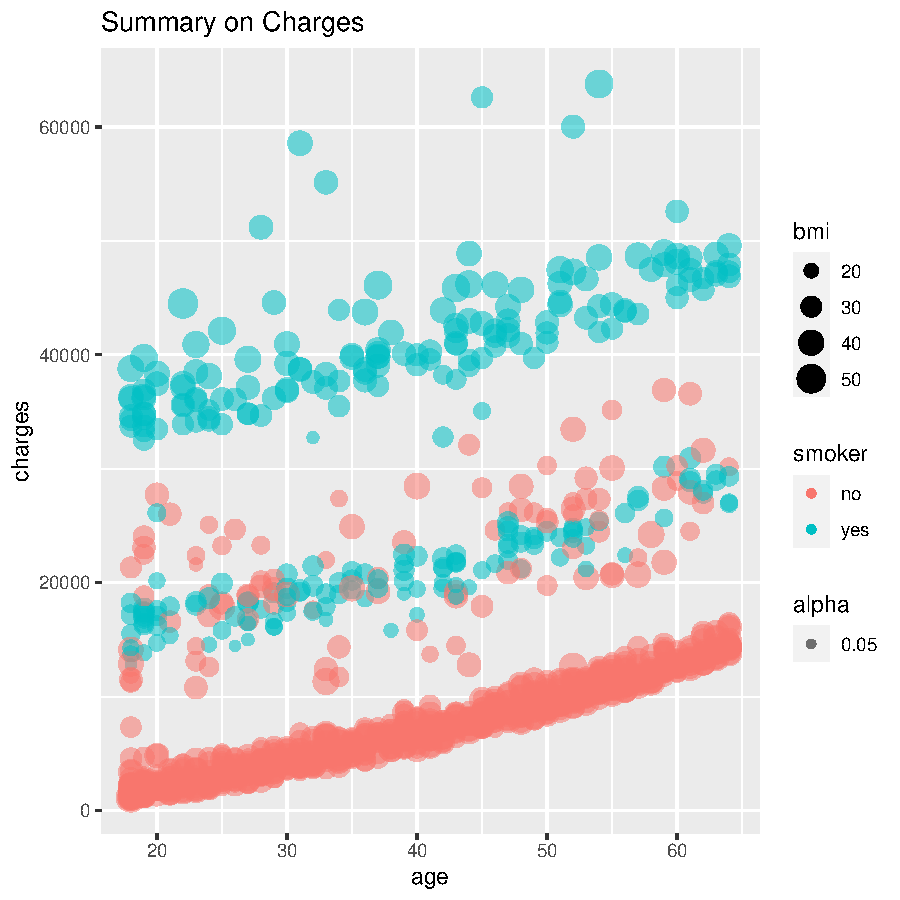
\includegraphics{Untitled-002}
\caption{Summary Plot}
\end{centerfig}

\begin{itemize}
  \item Koszty leczenia liniowo zaleza od wieku
  \item Koszty leczenia zaleza od tego, pali osoba czy nie. W przypadku osob palacych z "normalnym:" BMI (okolo 30), koszty leczenia sa 2 razy wieksze
niz dla osob niepalacych z normalnym BMI, natomiast obosy palace z wysokim albo bardzo nizkim BMI placa 4 razy wiecej niz osoby "zkwykle"
  \item Koszty leczenia zaleza od BMI, ale nie w takim wielkim stopniu, jak od palenia
  \item Koszty leczenia nie zaleza od plci.
\end{itemize}
Jako wynik badania powstaly kilka modeli, i nastepujaca byla wybrana przez autora jako najlepsza:
model<- lm (charges ~ age + smoker+ bmi + SmokerWithHighBMI,data), gdzie SmokerWithHighBMI to wartosc, wskazujaca, czy osoba pali i  ma BMI>30, albo nie w przeciwnym przypadku.
\ref{sec:Third}
\newline
Ten model daje p-value: < 2.2e-16, Adjusted R-squared: 0.8607, ale Residual Standard Error nie jest postaci normalnej.
Z pewnym przyblizeniem, mozna sie zgodzic na taki model.




\section{Data description}
Dane do projektu pochodza ze strony \href{url}{\texttt{https://www.kaggle.com/mirichoi0218/insurance}}. Skladaja sie z 1338 rekordow, zawierajacych nastepujaca informacje:
\begin{itemize}
  \item age: wiek beneficjenta pierwotnego
  \item sex: plec kontrahenta ubezpieczeniowego, kobieta, mezczyzna
  \item bmi: Wskaznik masy ciala, zapewniajacy zrozumienie ciala, masy, ktore sa stosunkowo wysokie lub niskie w stosunku do wzrostu,
  obiektywny wskaznik masy ciala \(kg/m^2\) na podstawie stosunku wzrostu do masy ciala, najlepiej 18,5 do 24,9
  \item children: Liczba dzieci objetych ubezpieczeniem zdrowotnym / Liczba osob na utrzymaniu
  \item smoker: Palenie
  \item region: obszar mieszkalny beneficjenta w USA, na polnocnym wschodzie, poludniowym wschodzie, poludniowym zachodzie i polnocnym zachodzie.
  \item charges: Indywidualne koszty leczenia rozliczane przez ubezpieczenie zdrowotne
\end{itemize}


\section{Analysis of single variables}
In this section we are going to perform analysis of single variables to discover their properties and to verify that data makes sens and is well-distributed.
\subsection{Smoking}
Let's take a look at plot of smokers:




\begin{centerfig}
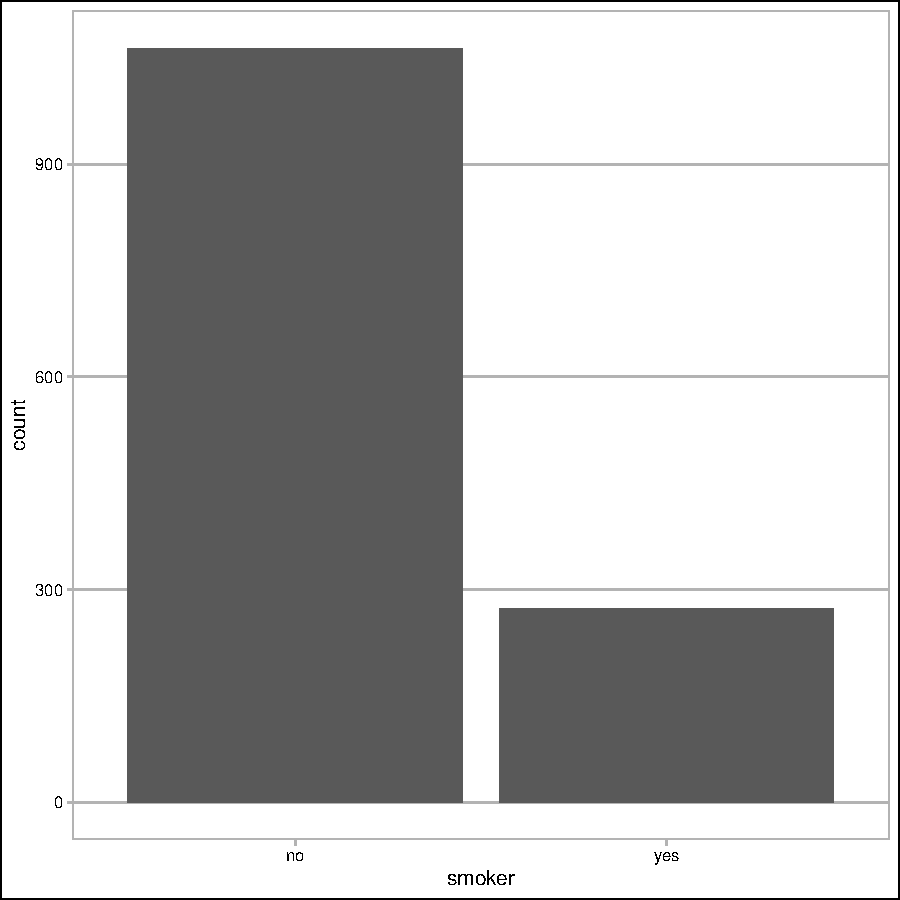
\includegraphics{Untitled-003}
\caption{Plot of smokers}
\end{centerfig}

As we can see, there are more smokers, than non-smokers, which applies us to be more carefull while making decision

\paragraph{Point Estimation of Population Proportion \newline} 
At this moment we can try to estimate the Proportion of smokers to non-smokers in America, having that small sample

\begin{Schunk}
\begin{Sinput}
> f = sum(data$smoker=='yes')
> n = length(data$smoker)
> f/n
\end{Sinput}
\begin{Soutput}
[1] 0.2047833
\end{Soutput}
\end{Schunk}

The point estimate of smoking people proportion in survey is 20\%, which is pretty close to our expectations (According to the CDC, as of 2015, a total of 15.1\% of U.S. adults (16.7\% of men and 13.6\% of women) smoke)

\subsection{Gender}

\begin{centerfig}
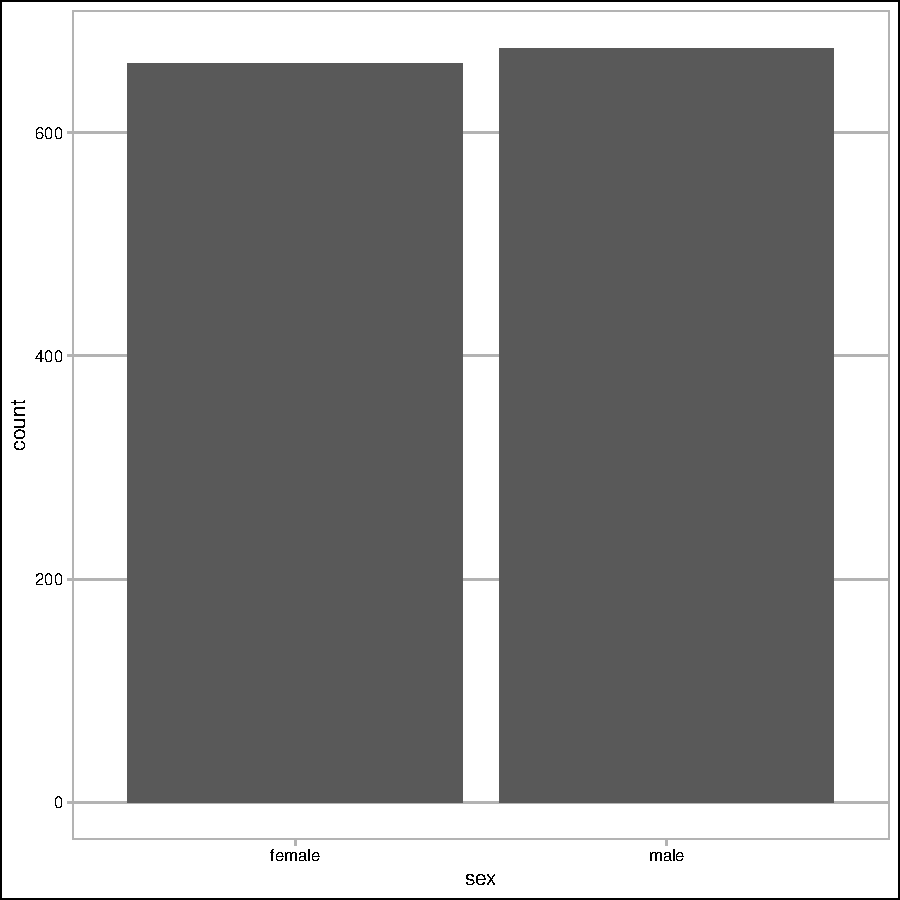
\includegraphics{Untitled-005}
\caption{Plot of genders}
\end{centerfig}
As we can see we have almost equal distribution of man and women in survey
\paragraph{Point Estimation of Gender Proportion \newline} 

\begin{Schunk}
\begin{Sinput}
>   f = sum(data$sex=='male')
>   n = length(data$sex)
>   f/n
\end{Sinput}
\begin{Soutput}
[1] 0.5052317
\end{Soutput}
\end{Schunk}

As we can see, the point estimate of male gender proportion in survey is 50\%, which also meets our expectations, meaning the data is accurate and well-distributed, comparing to population.

\subsection{Age}
\paragraph{Basic number properties \newline} 

\begin{Schunk}
\begin{Sinput}
> describeBy(data$age)
\end{Sinput}
\begin{Soutput}
   vars    n  mean    sd median trimmed   mad min max range skew kurtosis   se
X1    1 1338 39.21 14.05     39   39.01 17.79  18  64    46 0.06    -1.25 0.38
\end{Soutput}
\end{Schunk}
Analysing which, we can outline these properties:

\begin{itemize}
  \item[$-$] \textbf{n} - number of items
  \item[$-$] \textbf{mean} - mean of sample
  \item[$-$] \textbf{sd} - standard deviation ( a measure of the amount of variation)
  \item[$-$] \textbf{median} -  median of sample ( 50th percentile)
  \item[$-$] \textbf{trimmed} - trimmed mean, in other words this value is more stable than the mean, because it is calculated like:
    \begin{enumerate}
      \item Cut off 10\% from left side of distribution
      \item Cut off 10\% from right side of distribution
      \item Calculate average from the remaining 80\% 
    \end{enumerate}
  \item[$-$] \textbf{mad} - mean absolute deviation ( variability similar to the sum of squares)
  \item[$-$] \textbf{min} - minimum value
  \item[$-$] \textbf{max} - maximum value
  \item[$-$] \textbf{range} -  the difference between the max and min values
  \item[$-$] \textbf{skew} - \(A =\frac{\mu_3}{\sigma^3} \) a measure of asymmetry in the distribution
  \begin{enumerate}
    \item \( A==0 \Rightarrow\) distribution is symmetrical 
    \item \( A>0 \Rightarrow\) distribution has positive skew 
    \item \( A<0 \Rightarrow\) distribution negative skew 
    \end{enumerate}  
  \item[$-$] \textbf{kurtosis} - \(Kurt[X] = \frac{\mu_4}{\sigma^4}\) a measure of the peakedness of the probability distribution
    \begin{enumerate}
    \item \(Kurt[X]==0 \Rightarrow\) rounded peak of a normal distribution (Mesokurtic)
    \item \(Kurt[X]>0 \Rightarrow\) a sharper peak (Leptokurtic)
    \item \(Kurt[X]<0 \Rightarrow \) a flatter peak (Platykurtic)
    \end{enumerate}  
  \item[$-$] \textbf{se} - sample standard error
\end{itemize}

\paragraph{Average deviation \newline} 

\begin{Schunk}
\begin{Sinput}
> avg.dev <- function(x)
+   mean(abs(x - mean(x)))
> c(avg.dev(data$age))
\end{Sinput}
\begin{Soutput}
[1] 12.24893
\end{Soutput}
\end{Schunk}

\paragraph{Quantiles (minimum, lower-hinge, median, upper-hinge, maximum) \newline} 
\begin{Schunk}
\begin{Sinput}
> fivenum(data$age)
\end{Sinput}
\begin{Soutput}
[1] 18 27 39 51 64
\end{Soutput}
\end{Schunk}

\paragraph{(upper-hinge - lower-hinge) \newline} 
\begin{Schunk}
\begin{Sinput}
> IQR(data$age)
\end{Sinput}
\begin{Soutput}
[1] 24
\end{Soutput}
\end{Schunk}

\paragraph{Central, not absolute moments \newline} 
\begin{Schunk}
\begin{Sinput}
> moment(data$age,0.25)
\end{Sinput}
\begin{Soutput}
[1] 2.469482
\end{Soutput}
\begin{Sinput}
> moment(data$age,0.5)
\end{Sinput}
\begin{Soutput}
[1] 6.154262
\end{Soutput}
\begin{Sinput}
> moment(data$age,0.75)
\end{Sinput}
\begin{Soutput}
[1] 15.47053
\end{Soutput}
\begin{Sinput}
> moment(data$age,1)
\end{Sinput}
\begin{Soutput}
[1] 39.20703
\end{Soutput}
\end{Schunk}



\paragraph{Plots \newline} 
Below we can see different types of plots to help us in analyzing the sample.
\begin{centerfig}
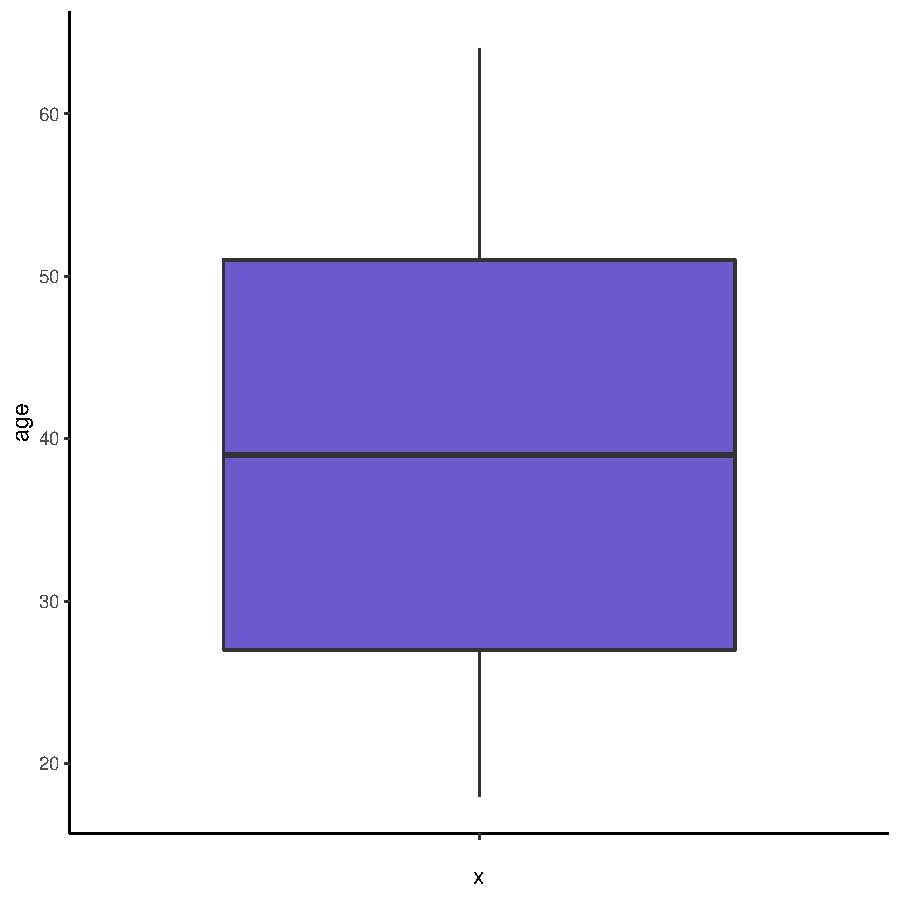
\includegraphics{Untitled-012}
\caption{BoxPlot of age}
\end{centerfig}

\begin{centerfig}
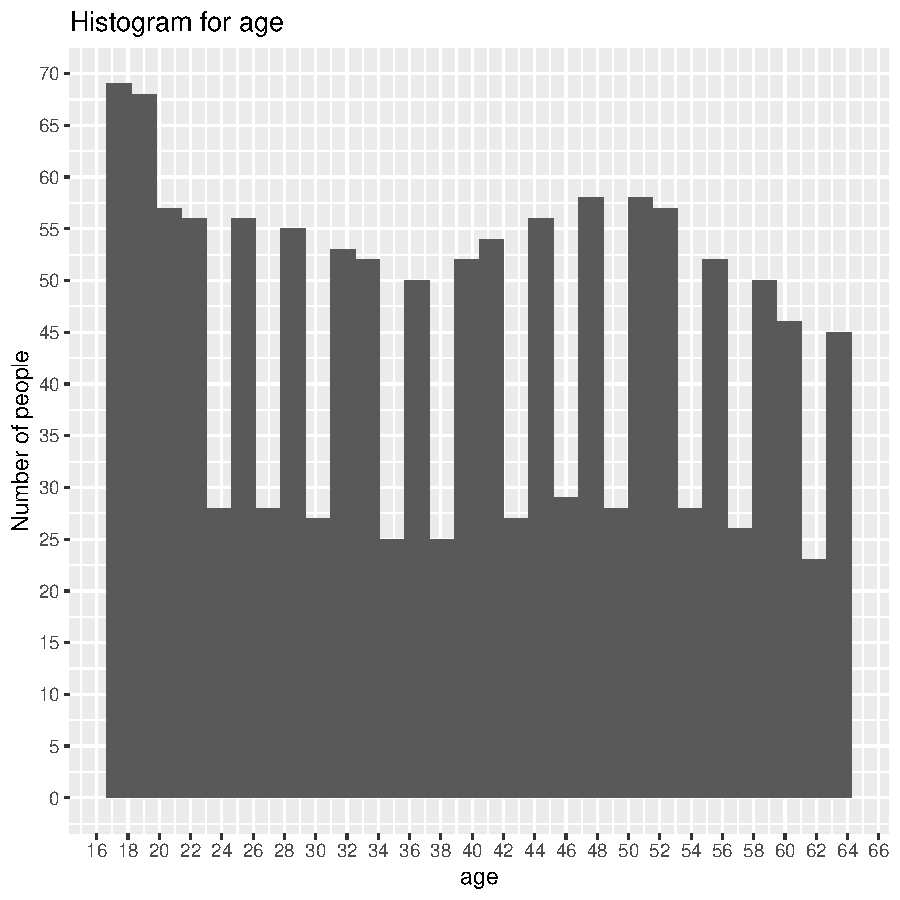
\includegraphics{Untitled-013}
\caption{Histogram of age}
\end{centerfig}

\begin{centerfig}
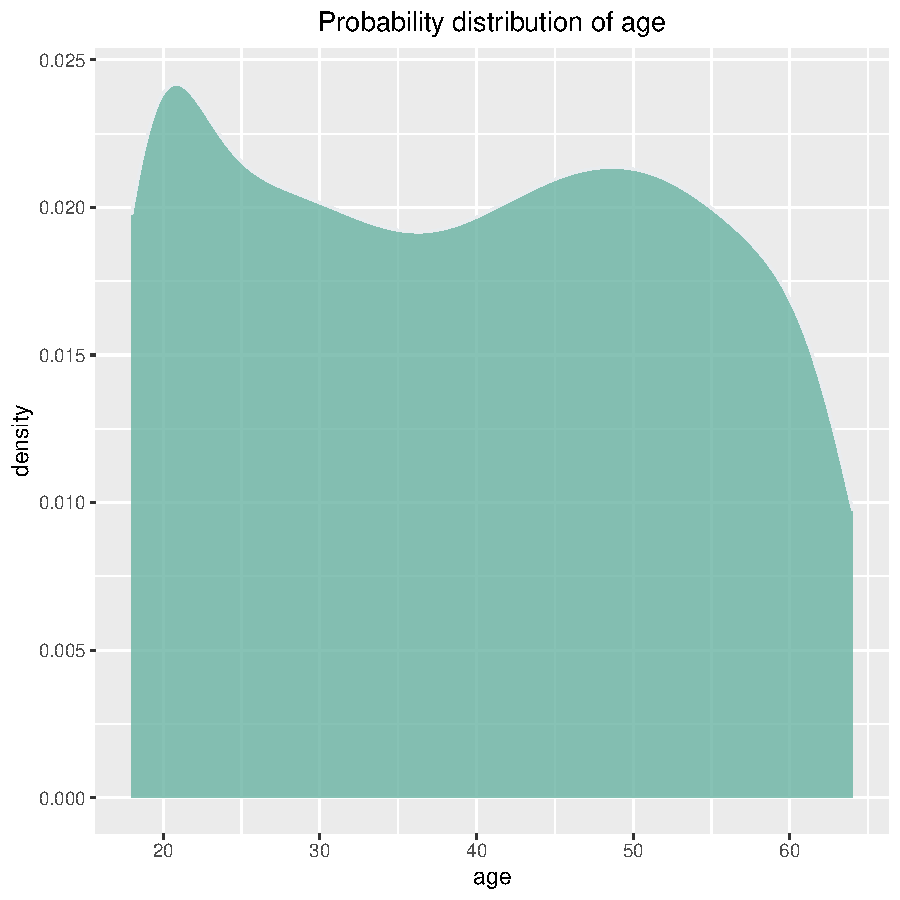
\includegraphics{Untitled-014}
\caption{Probability distribution of age}
\end{centerfig}

As we can see, we've got evenly uniformly distributed variable, 
So next analysis can pretend to be accurate



\subsection{Testing BMI distribution}
\paragraph{Basic number properties \newline} 
\begin{Schunk}
\begin{Sinput}
> describeBy(data$bmi)
\end{Sinput}
\begin{Soutput}
   vars    n  mean  sd median trimmed mad   min   max range skew kurtosis   se
X1    1 1338 30.66 6.1   30.4    30.5 6.2 15.96 53.13 37.17 0.28    -0.06 0.17
\end{Soutput}
\end{Schunk}
Analysing which, we can outline the same properties as in previous one.
\paragraph{Average deviation \newline} 

\begin{Schunk}
\begin{Soutput}
[1] 4.897871
\end{Soutput}
\end{Schunk}
\paragraph{Quantiles (minimum, lower-hinge, median, upper-hinge, maximum) \newline} 
\begin{Schunk}
\begin{Soutput}
[1] 15.96 26.29 30.40 34.70 53.13
\end{Soutput}
\end{Schunk}

\paragraph{ (upper-hinge - lower-hinge) \newline} 
\begin{Schunk}
\begin{Soutput}
[1] 8.3975
\end{Soutput}
\end{Schunk}

\paragraph{ Central, not absolute moments \newline} 
\begin{Schunk}
\begin{Soutput}
[1] 2.344357
\end{Soutput}
\begin{Soutput}
[1] 5.509917
\end{Soutput}
\begin{Soutput}
[1] 12.98222
\end{Soutput}
\begin{Soutput}
[1] 30.6634
\end{Soutput}
\end{Schunk}

\paragraph{Plots \newline} 
Below we can see different types of plots to help us in analyzing the sample.

\begin{centerfig}
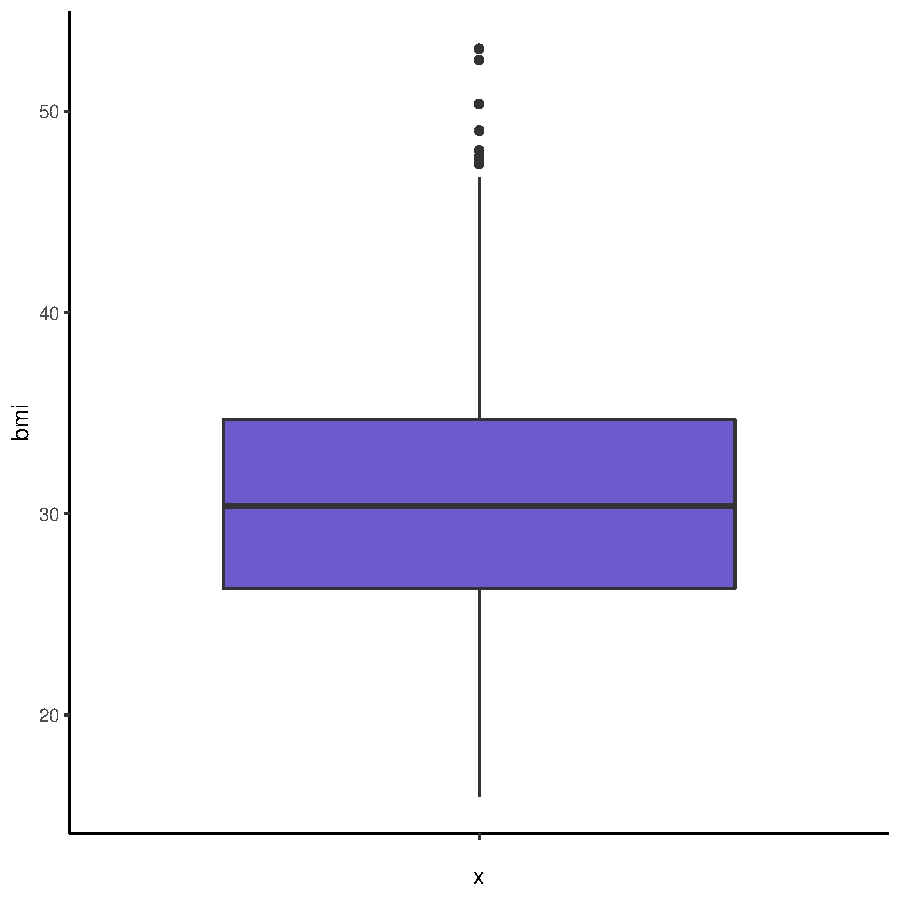
\includegraphics{Untitled-020}
\caption{BoxPlot of bmi}
\end{centerfig}

\begin{centerfig}
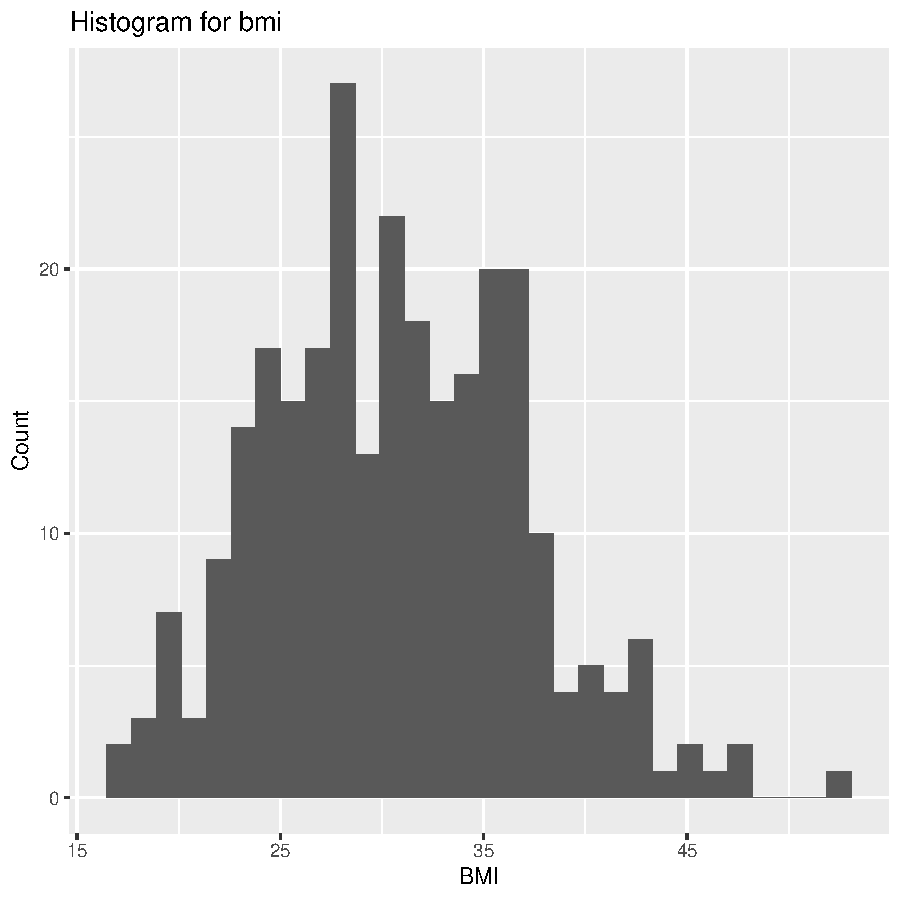
\includegraphics{Untitled-021}
\caption{Histogram of bmi}
\end{centerfig}

\begin{centerfig}
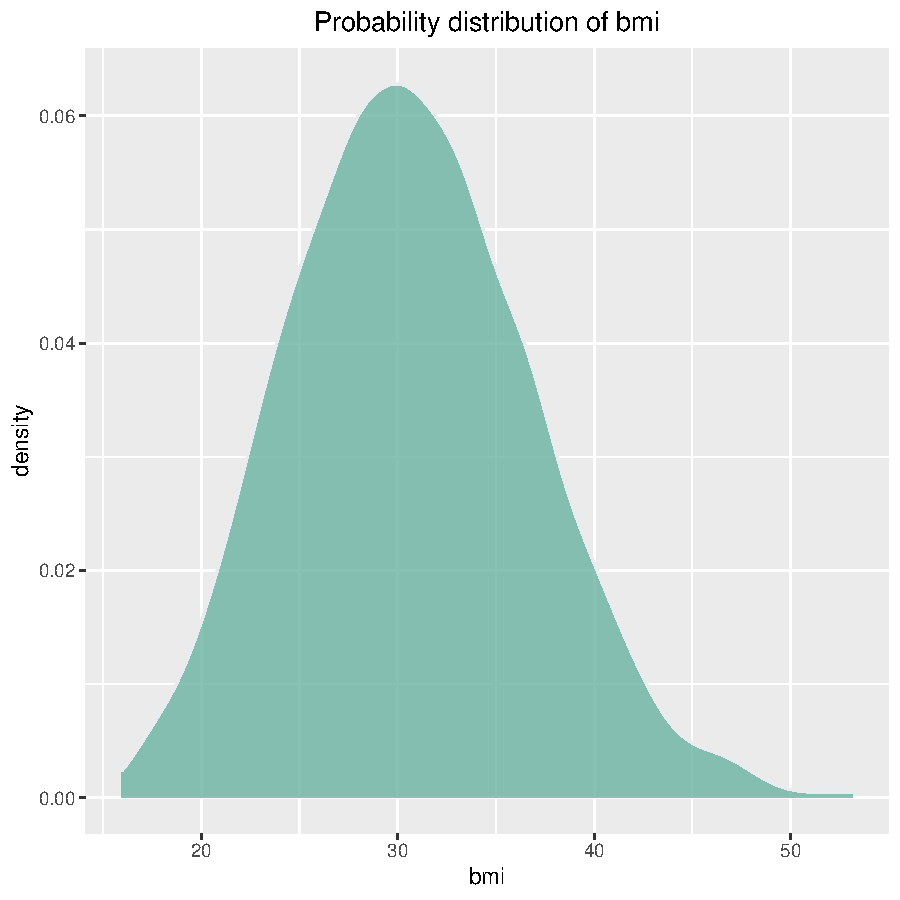
\includegraphics{Untitled-022}
\caption{Probability distribution of bmi}
\end{centerfig}

As we can see, we've got something that looks like normal distribution,
so let's take a closer look at it.

\paragraph{Visual methods -> Density plot of BMI\newline}

\begin{centerfig}
\begin{Schunk}
\begin{Sinput}
> ggplot( data, aes(x=bmi)) +
+   geom_density(fill="#69b3a2", color="#e9ecef", alpha=0.8) +
+   ggtitle("Probability distribution of bmi") +
+   theme(plot.title = element_text(hjust = 0.5))
\end{Sinput}
\end{Schunk}
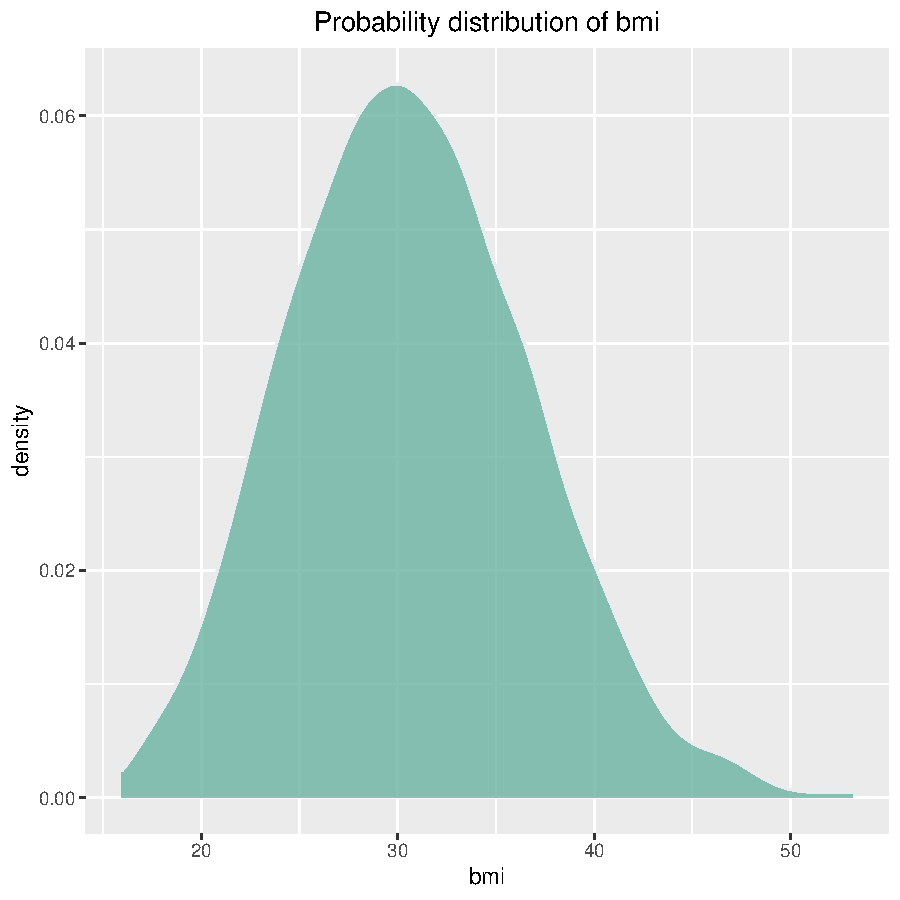
\includegraphics{Untitled-023}
\caption{Density plot of BMI}
\end{centerfig}

The plot looks like normal, so continue our analyzing, now using qqplot:

\begin{centerfig}
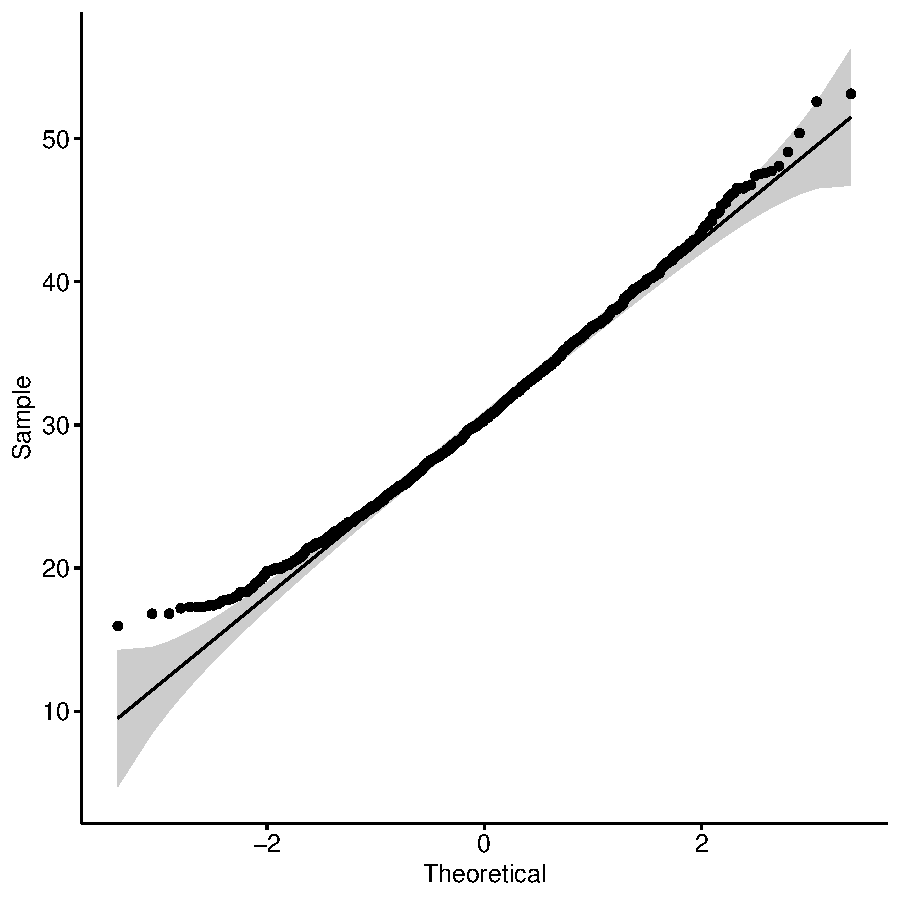
\includegraphics{Untitled-024}
\caption{Plot of BMI}
\end{centerfig}

As we can see there, at the begining there is small deviation from line of normal distribution, but still it's worth testing.


\subsection{Children}
Let's see whether charges depend on children
\begin{centerfig}
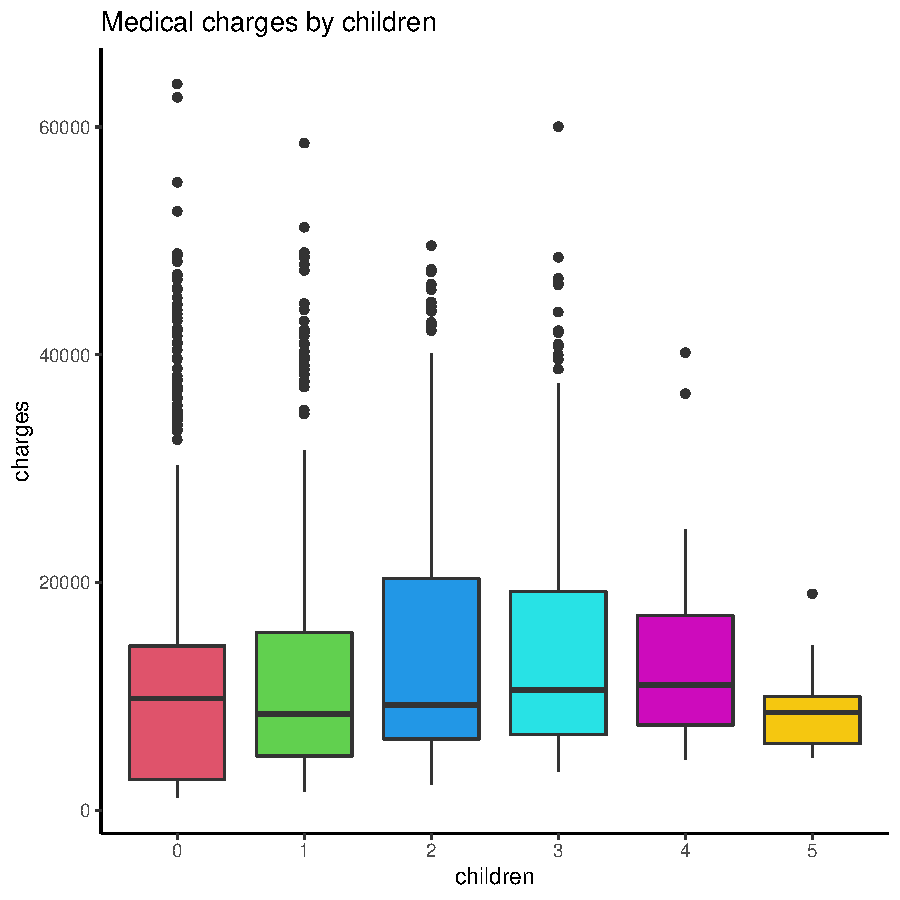
\includegraphics{Untitled-025}
\caption{Charges on children}
\end{centerfig}


\subsection{Charges}

\paragraph{Basic number properties \newline} 

\begin{Schunk}
\begin{Sinput}
> describeBy(data$charges)
\end{Sinput}
\begin{Soutput}
   vars    n     mean       sd  median  trimmed     mad     min      max
X1    1 1338 13270.42 12110.01 9382.03 11076.02 7440.81 1121.87 63770.43
      range skew kurtosis     se
X1 62648.55 1.51     1.59 331.07
\end{Soutput}
\end{Schunk}

\paragraph{Average deviation \newline} 

\begin{Schunk}
\begin{Soutput}
[1] 9091.127
\end{Soutput}
\end{Schunk}
\paragraph{Quantiles (minimum, lower-hinge, median, upper-hinge, maximum) \newline} 
\begin{Schunk}
\begin{Soutput}
[1]  1121.874  4738.268  9382.033 16657.717 63770.428
\end{Soutput}
\end{Schunk}

\paragraph{ (upper-hinge - lower-hinge) \newline} 
\begin{Schunk}
\begin{Soutput}
[1] 11899.63
\end{Soutput}
\end{Schunk}

\paragraph{ Central, not absolute moments \newline} 
\begin{Schunk}
\begin{Soutput}
[1] 9.982301
\end{Soutput}
\begin{Soutput}
[1] 104.8336
\end{Soutput}
\begin{Soutput}
[1] 1154.389
\end{Soutput}
\begin{Soutput}
[1] 13270.42
\end{Soutput}
\end{Schunk}

\paragraph{Plots \newline} 
Below we can see different types of plots to help us in analyzing the sample.

\begin{centerfig}
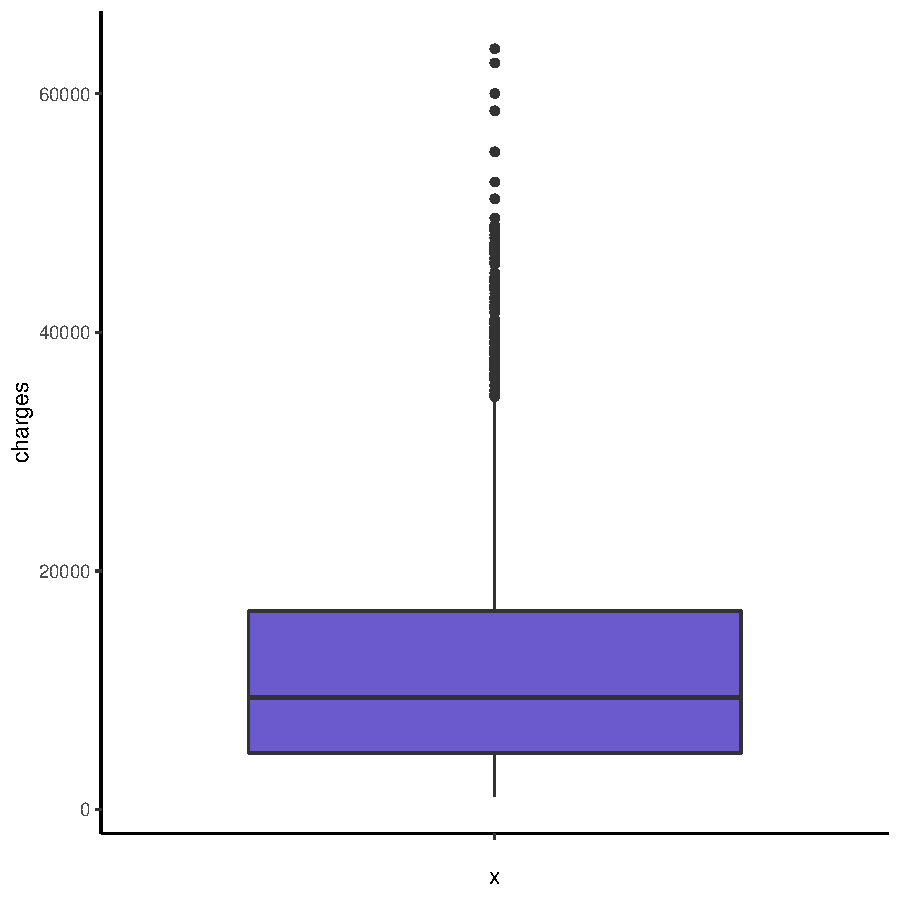
\includegraphics{Untitled-031}
\caption{BoxPlot of charges}
\end{centerfig}

\begin{centerfig}
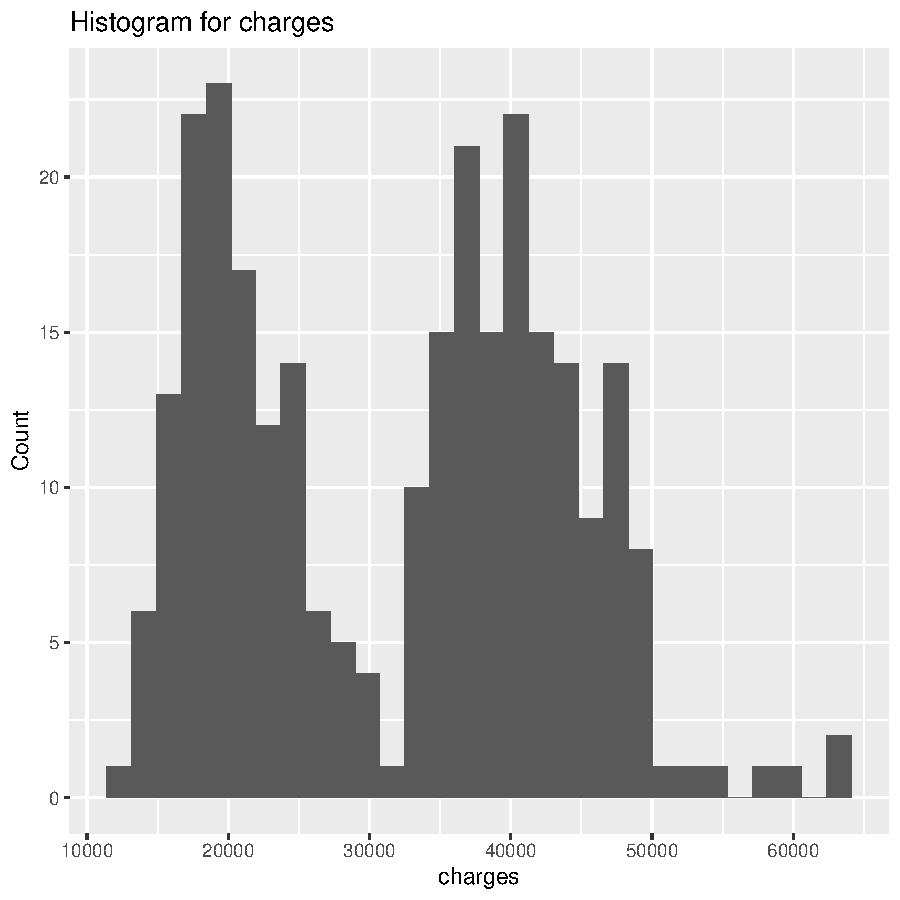
\includegraphics{Untitled-032}
\caption{Histogram of charges}
\end{centerfig}

\begin{centerfig}
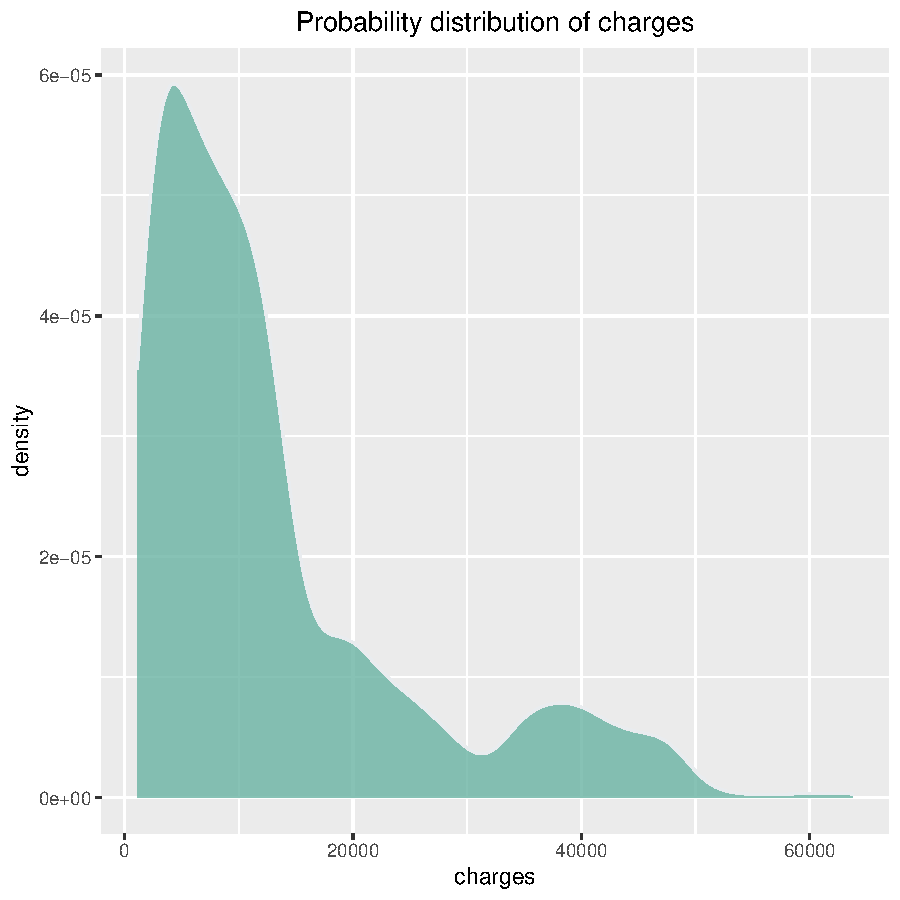
\includegraphics{Untitled-033}
\caption{Probability distribution of charges}
\end{centerfig}


\section{Testing}



\subsection{Quick Theory Review on Testing}
\paragraph{Two-samples t-test\newline}
In t-test, the null hypothesis is that the mean of the two samples is equal.
So the alternative hypothesis is that the means are different or, \(|m_1 - m_2| > 0\)
So basically, we want to take or reject the null hypothesis with some confidence interval (the range of values within which the difference may lie)
Also, t-test gives us a \(p-value\), probability of us, making wrong decision
Having small \(p-value\) suggests having small probability for null-hypothesis being true.

\paragraph{Shapiro-Wilk’s method\newline}
Method, based on correlation between the data and the corresponding "normal points"
Null-hypothesis is that distribution is normal and we reject the null hypothesis if p < 0.05, meaning that distribution is more likely not normal.
Wilk’s test should not be significant to meet the assumption of normality.

\paragraph{One-sample t-test\newline}
Assumptions:
\begin{itemize}
  \item Population is normally distributed
  \item Independent samples
  \item Random sample via all population distribution
  \item Continuous
  \end{itemize}
Defining null-hypothesis, we assume that mean of our population is equal to a hypothezed value



\subsection{Is BMI Normally Distributed?}
In the case of BMI, we can see some outliers, and it can be a point where we stop testing and say that the model doesn't meet the Assumptions, but we will go further.
\newline

First of all let's apply Shapiro-Wilk’s test (assuming that Assumptions are met)

\begin{Schunk}
\begin{Sinput}
> shapiro.test(data$bmi)
\end{Sinput}
\begin{Soutput}
	Shapiro-Wilk normality test

data:  data$bmi
W = 0.99389, p-value = 2.605e-05
\end{Soutput}
\end{Schunk}

Having p-value = 2.605e-05, we can reject the null hypothesis, that distribution is normal, applying from that non-normality of our sample distribution.


Also we can try t-test, with default arguments:
\newline
\begin{Schunk}
\begin{Sinput}
> t.test(data$bmi, y = NULL,
+        alternative = c("two.sided", "less", "greater"),
+        mu = 0, paired = FALSE, var.equal = FALSE,
+        conf.level = 0.95)
\end{Sinput}
\begin{Soutput}
	One Sample t-test

data:  data$bmi
t = 183.93, df = 1337, p-value < 2.2e-16
alternative hypothesis: true mean is not equal to 0
95 percent confidence interval:
 30.33635 30.99045
sample estimates:
mean of x 
  30.6634 
\end{Soutput}
\end{Schunk}

Having tested with t.test (p-value < 2.2e-16) we can conclude that it's highly significant that BMI is not distributed normally

\paragraph{Density Estimate of data \newline}
\begin{centerfig}
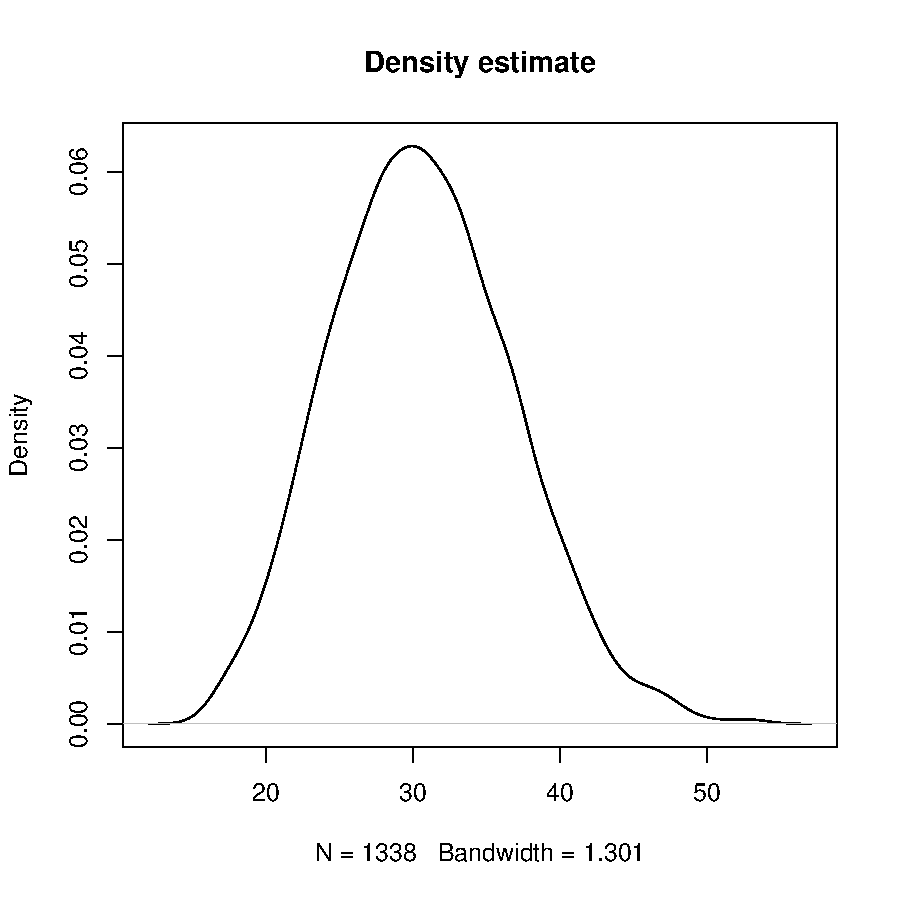
\includegraphics{Untitled-036}
\caption{Dencity estimaate}
\end{centerfig}

\subsection{Do charges depend on gender?}


\begin{Schunk}
\begin{Sinput}
> mans_charge <- subset(data,sex=="male" & smoker=='no')
> females_charge <- subset(data,sex=="female"& smoker=='no')
\end{Sinput}
\end{Schunk}

As we see on boxplots below, visually they have the same distribution, and median

\begin{centerfig}
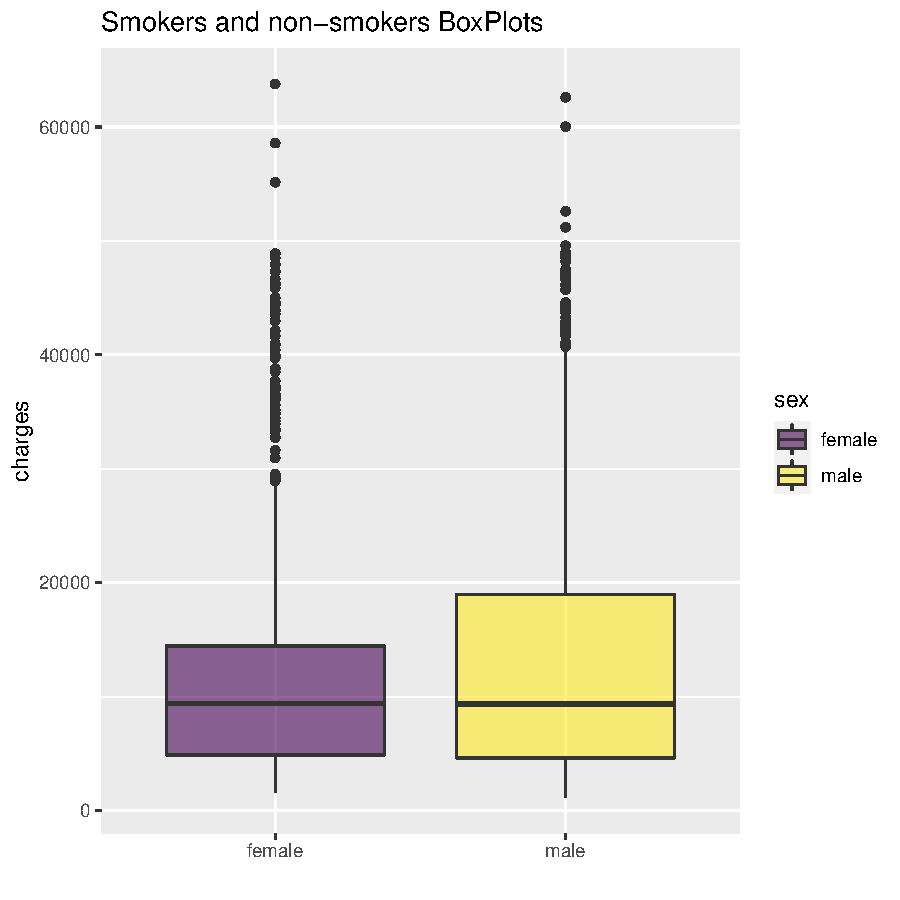
\includegraphics{Untitled-038}
\caption{BoxPlot of Smokers and non-smokers}
\end{centerfig}

Let's show it using t-test

First check for assumptions:
Distribution is not normal, so we need to stop in there, but we will continue due to insterest, understanding that we can't conclude anything from this testing

\begin{Schunk}
\begin{Sinput}
> test <- t.test( mans_charge$charges, females_charge$charges
+ )
> test
\end{Sinput}
\begin{Soutput}
	Welch Two Sample t-test

data:  mans_charge$charges and females_charge$charges
t = -1.8396, df = 1061, p-value = 0.0661
alternative hypothesis: true difference in means is not equal to 0
95 percent confidence interval:
 -1395.16882    44.98368
sample estimates:
mean of x mean of y 
 8087.205  8762.297 
\end{Soutput}
\end{Schunk}

So because p-value is < 0.07 we could assume (if distribution was normal)right that they are from same population. Which would mean that it doesn't matter which gender is the person, whose charge we are analysing.



\section{Interval Estimators for single variables}

\subsection{BMI}

We will use The One Sample t Test -> determines whether the sample mean is statistically different from a known or hypothesized population mean. Assumptions where discussed previously, so let's just check them:
\begin{itemize}
  \item \textbf{Independent} - OK
  \item \textbf{Random} - OK
  \item \textbf{Continuous} - OK
  \item \textbf{Normally distributed} - According to Shapiro-Wilk’s test, formally, we don't have normally distributed BMI, so we can't apply t-test, but because difference between our distribution and normal is acceptably small, let's assume normality
  \end{itemize}

\begin{Schunk}
\begin{Sinput}
> t.test(data$bmi)
\end{Sinput}
\begin{Soutput}
	One Sample t-test

data:  data$bmi
t = 183.93, df = 1337, p-value < 2.2e-16
alternative hypothesis: true mean is not equal to 0
95 percent confidence interval:
 30.33635 30.99045
sample estimates:
mean of x 
  30.6634 
\end{Soutput}
\end{Schunk}
Our confidence interval is [30.33635, 30.99045], mean of x is 30.6634 and p-value < 2.2e-16, meaning, that we can reject null-hypothesis, that sample and population having same mean, and accept alternative, that means are different and mean of population lies in [30.33635, 30.99045] with probability of 95 percent

Now let's make some calculus by ourselves and see, can we get the same result:
\newline
Math part:
\begin{itemize}
  \item \textbf{n} - number of elements in sample
  \item \textbf{\(\mu = \frac{1}{n}\sum_{i=1}^{n}(x_i)\)} - mean of sample
  \item \textbf{\(\sigma = \sqrt{\sigma^2}\)} - standard deviation
  \item \textbf{\(\sigma_{x} = \frac{\sigma}{sqrt(n)}\)} - standard error
  \item \textbf{\(z = \Phi(0.025)\)} - critical value Z, normal distribution in 0.025 (As we want to get 95\% interval of confidence, we need to take 2.5\% from left and right)
  \item \textbf{\([l=\mu-z*\sigma_{x},r = \mu+z* \sigma_{x}]\)} - Confidence interval 
  \end{itemize}
R part:
\begin{Schunk}
\begin{Sinput}
> n <- length(data$bmi)
> mu <- mean(data$bmi)
> s <- sd(data$bmi)
> err <- s/sqrt(n)
> z <- qnorm(0.025, lower.tail = F) 
> lower_ci <- mu - z*err
> upper_ci <- mu + z*err
> interval_estimation <- c("estimate" = mu, "lower95%" = lower_ci, "upper95%" = upper_ci)
> round(interval_estimation, digits = 5)
\end{Sinput}
\begin{Soutput}
estimate lower95% upper95% 
30.66340 30.33664 30.99015 
\end{Soutput}
\end{Schunk}

\section{Dependencies between data samples}

Now let's check for dependencies. First of all build Correlogram to find out correlation dependencies

\begin{centerfig}
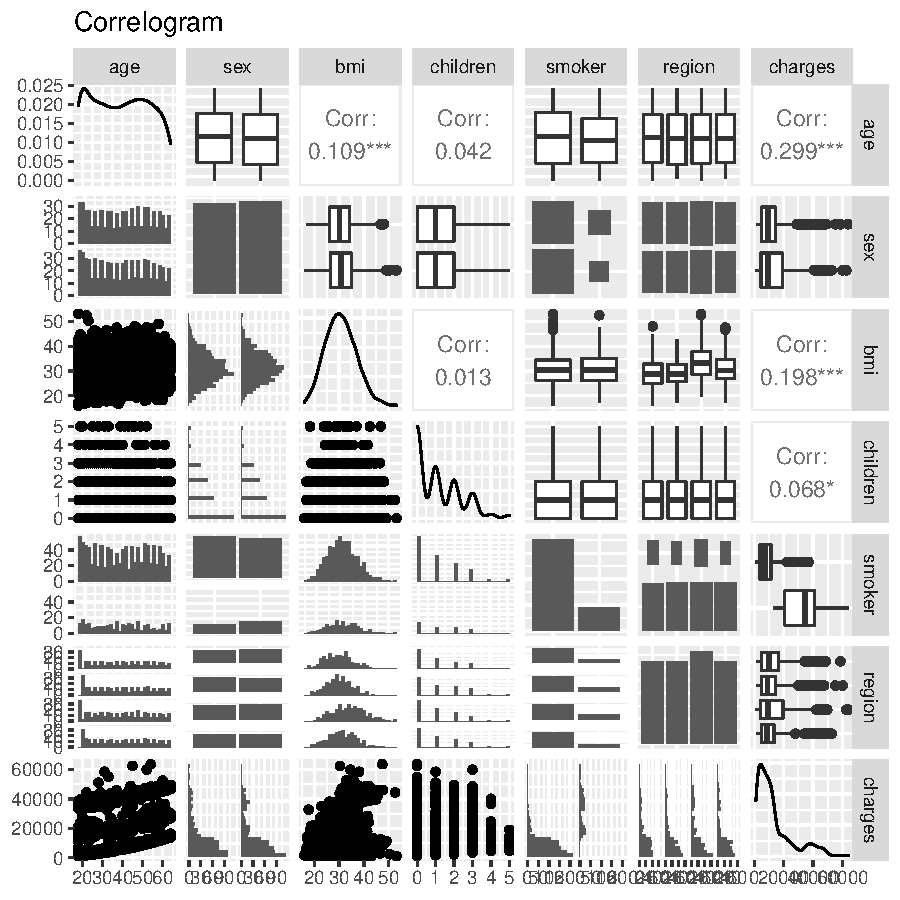
\includegraphics{Untitled-042}
\caption{Correlogram}
\end{centerfig}

\begin{centerfig}
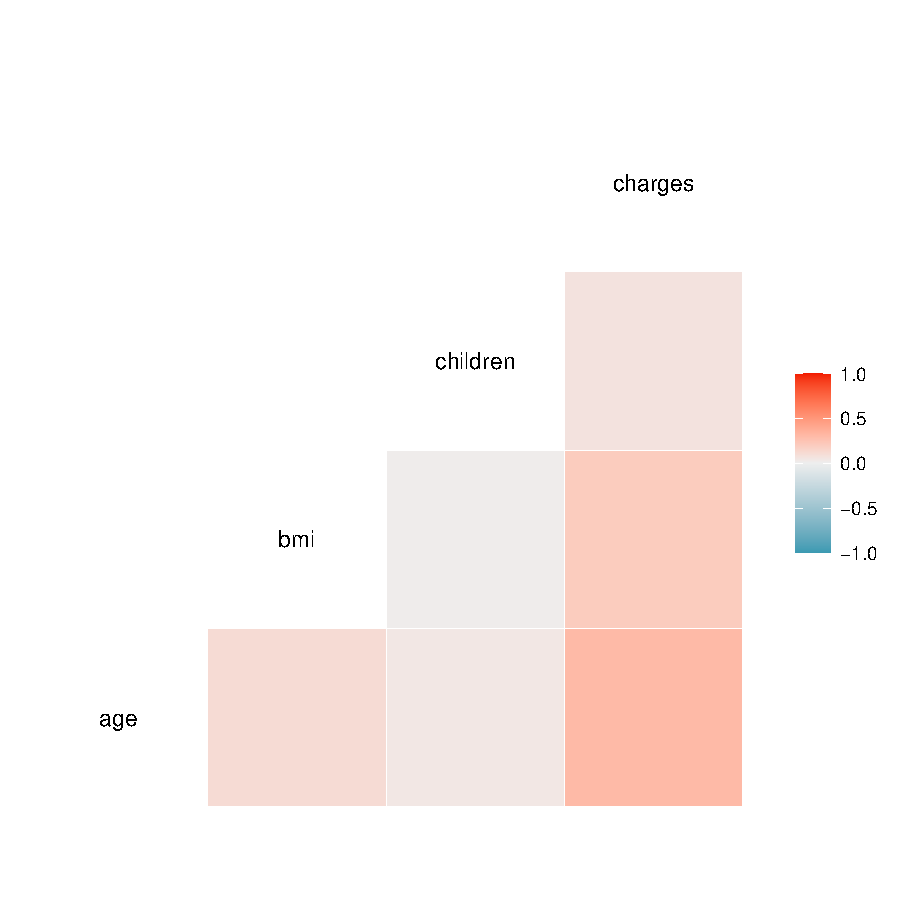
\includegraphics{Untitled-043}
\caption{Correlation}
\end{centerfig}

As we can see, the  age has the highest correlation with charges (0.299)***,
Also BMI has (0.198)*** correlation, which can give us some expectancies to 
Future, where *** means Pr(>|t|) close to 0

\subsection{Smoking and charges}

Looks like we have more smokers than non-smokers, lets have a look
How it affects out charge statistics

\begin{centerfig}
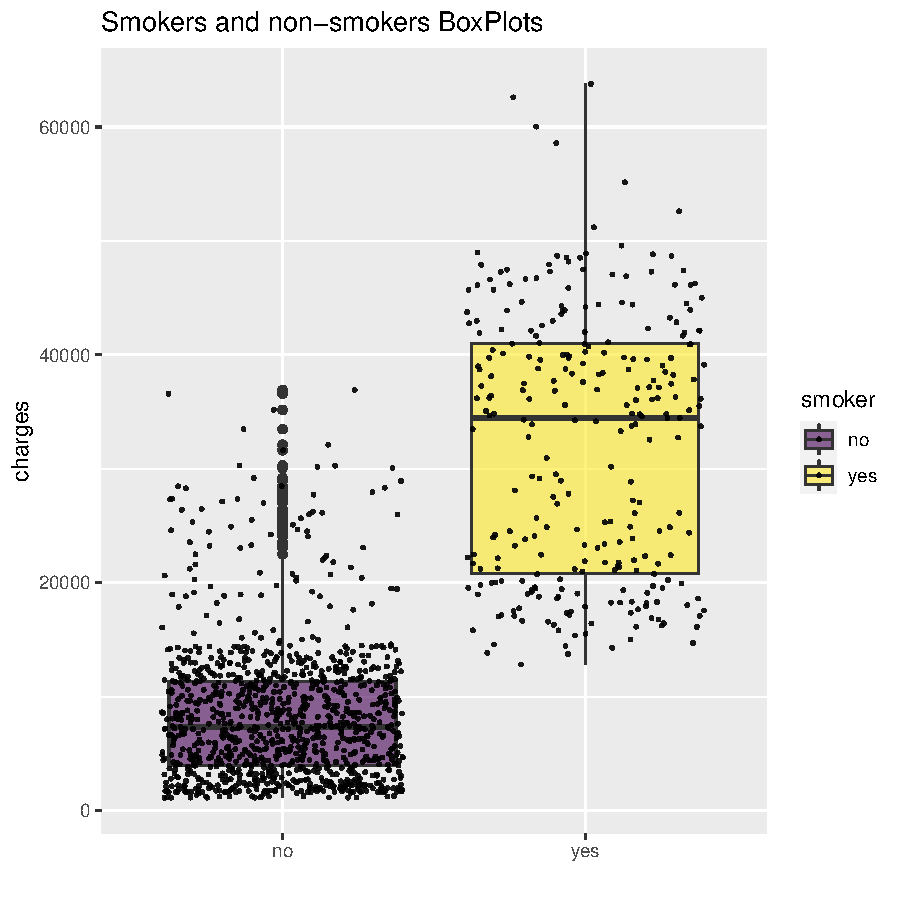
\includegraphics{Untitled-044}
\caption{BoxPLot on smoking}
\end{centerfig}

Looks like more data about non-smokers doesn't change the picture, 
but we can trust it more
And we can visually divide data from smokers into 2 groups, lets find out 
why


\begin{centerfig}
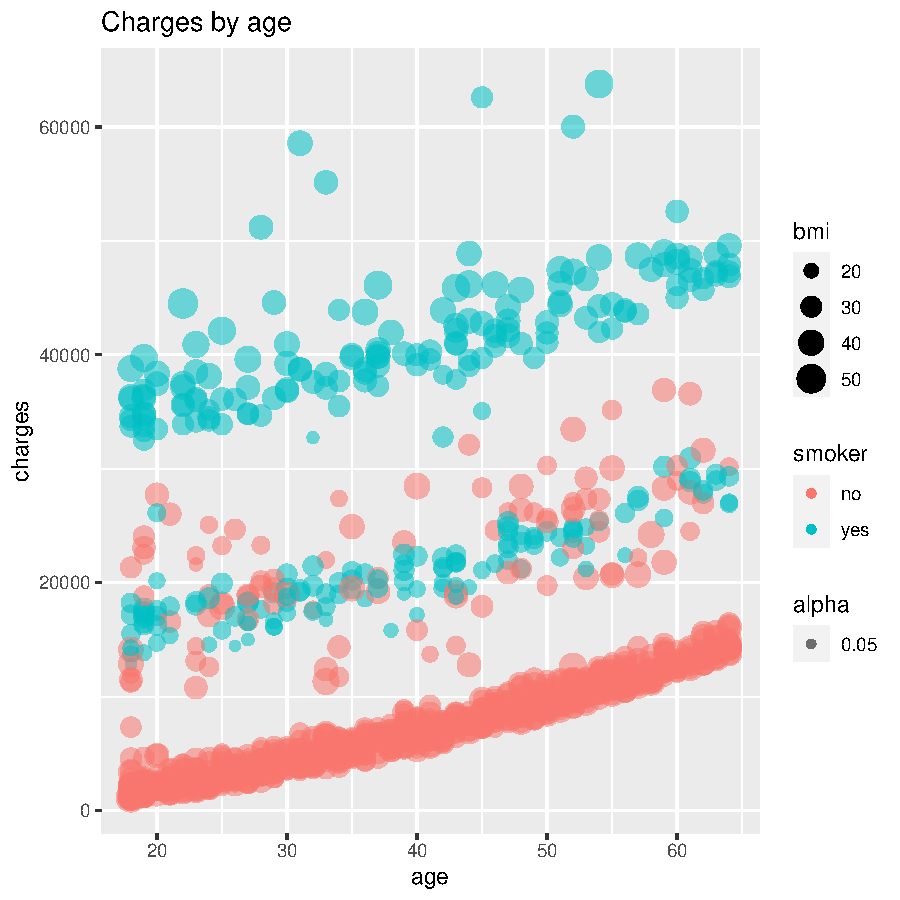
\includegraphics{Untitled-045}
\caption{Age and Charges}
\end{centerfig}

From that we can find out that smokers with high BMI pay more than smokers with low
Also there looks like a linear dependency between age and charges, but we will find it out later

So lets plot the age and the charges for non-smokers

\begin{centerfig}
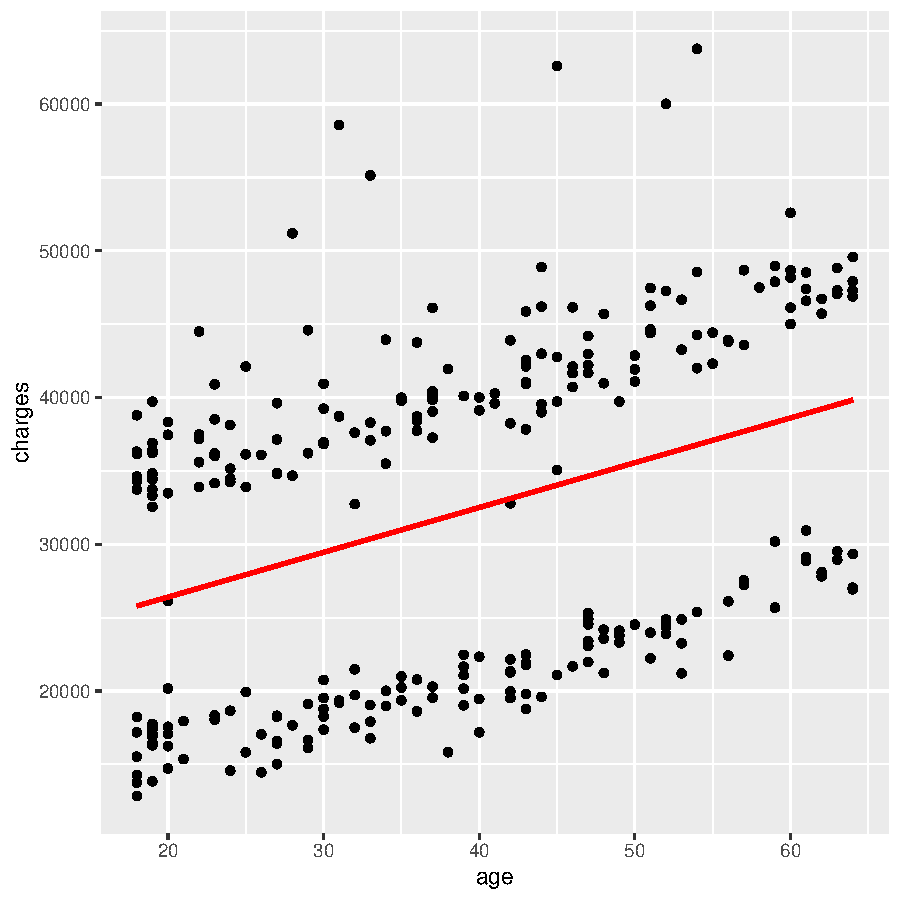
\includegraphics{Untitled-046}
\caption{Plot of age and charges}
\end{centerfig}

So we can see that charges are greater, as a line-dependency is visually rising faster

Now lets for our interest find out at what age is the most 'smoker' age

\begin{centerfig}
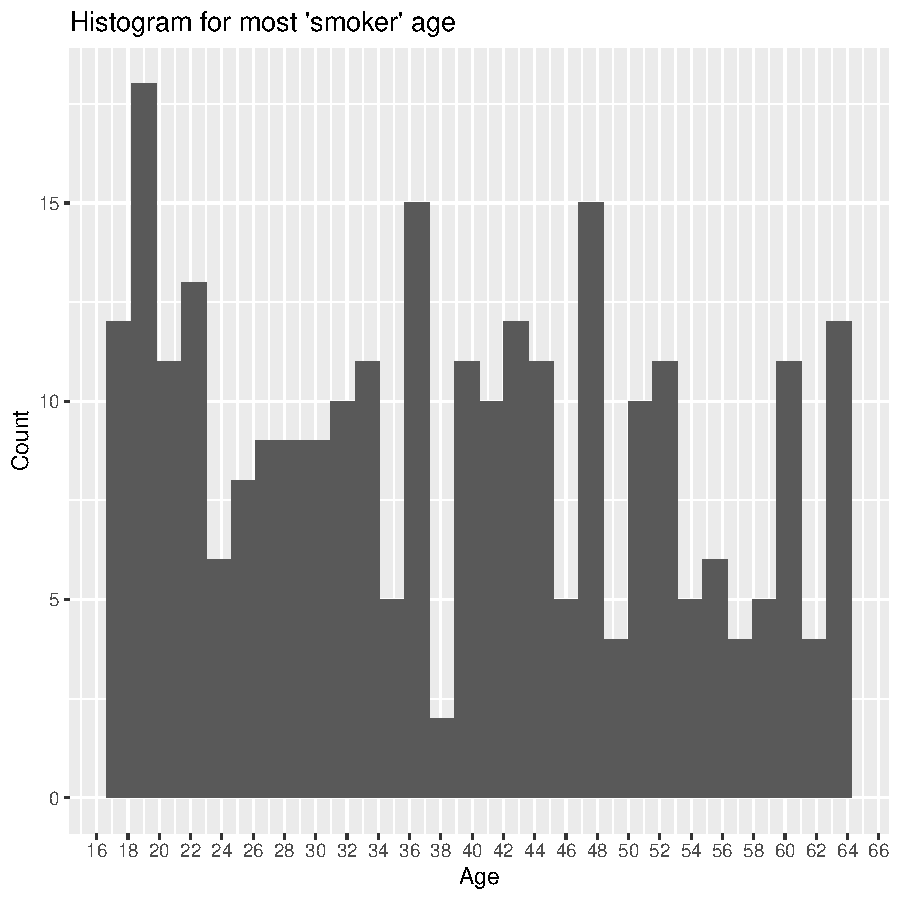
\includegraphics{Untitled-047}
\caption{Histogram for most 'smoker' age"}
\end{centerfig}

So around 19 is the most smoking age (based on our data)

\begin{centerfig}
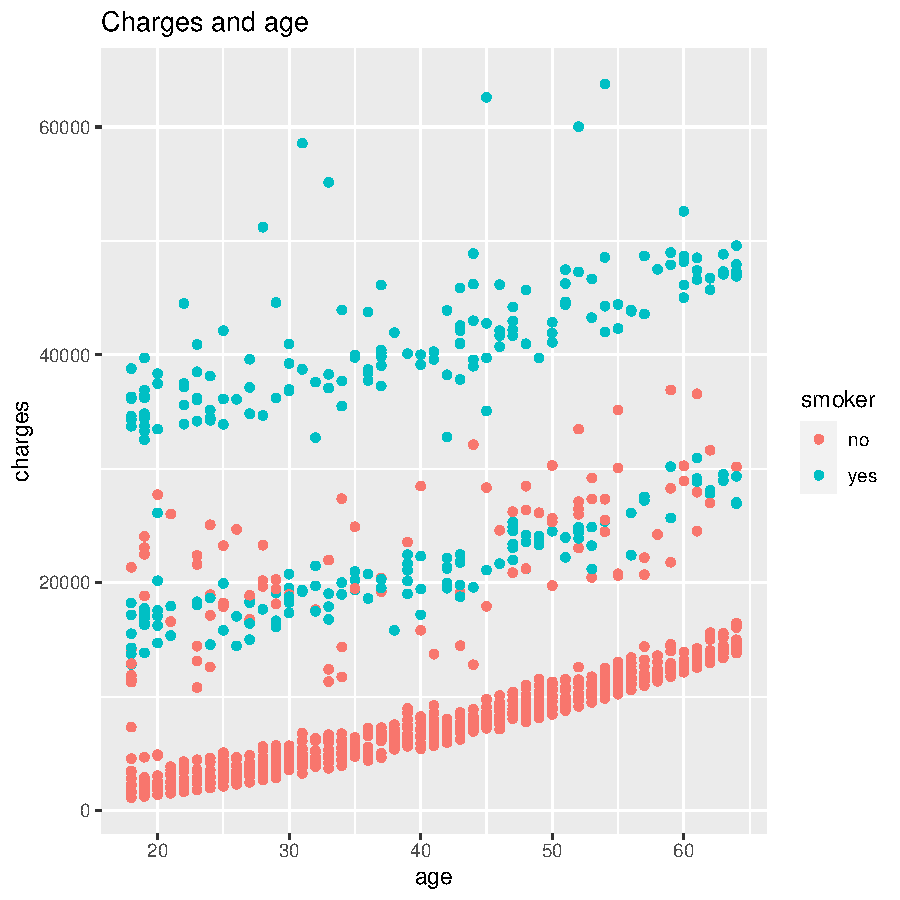
\includegraphics{Untitled-048}
\caption{Charges on age}
\end{centerfig}

Summing up on smoking

So based on the analysis we can say, that smokers in average pay more for treatment
then non-smokers, smokers can be divided into two groups - those with normal BMI (~30)
and those with high BMI, the second group is more affected by deceases and in
the end pays more for treatment. (Or insurance is more in our case)


\subsection{Gender and charges}

Let's see is gender connected with charges

\begin{centerfig}
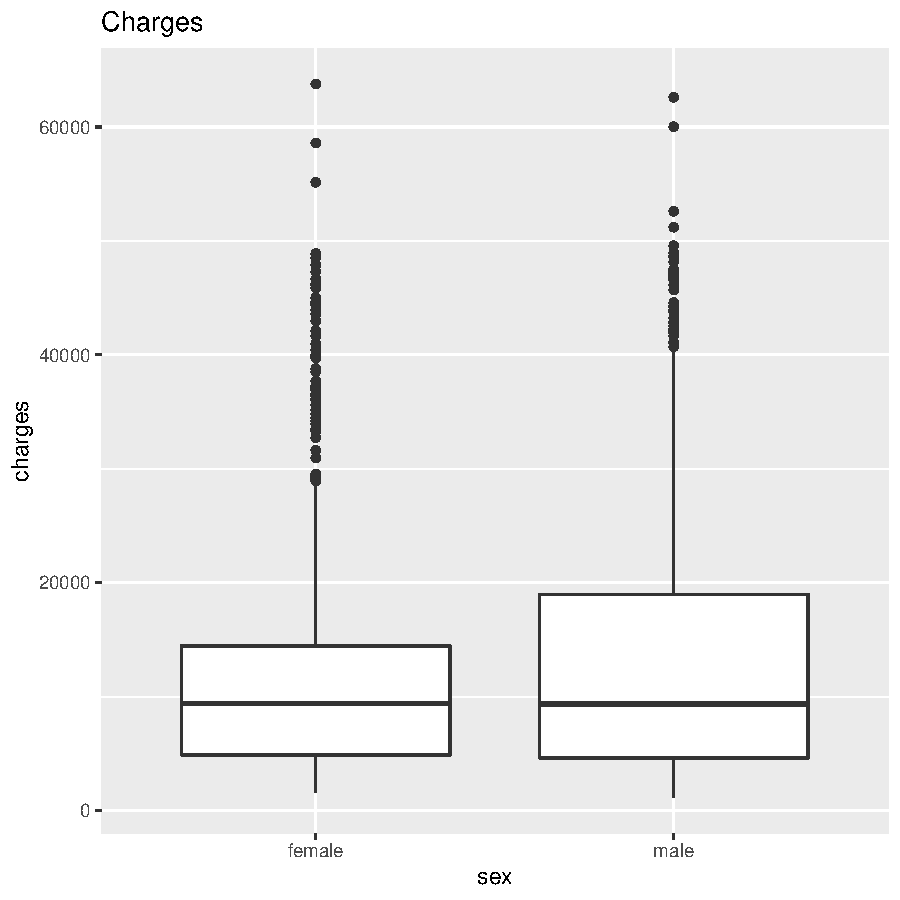
\includegraphics{Untitled-049}
\caption{Gender and charges}
\end{centerfig}

So it's not correlated, and gender doesn't affect charges

\subsection{BMI and charges}
Summing up we have 

\begin{centerfig}
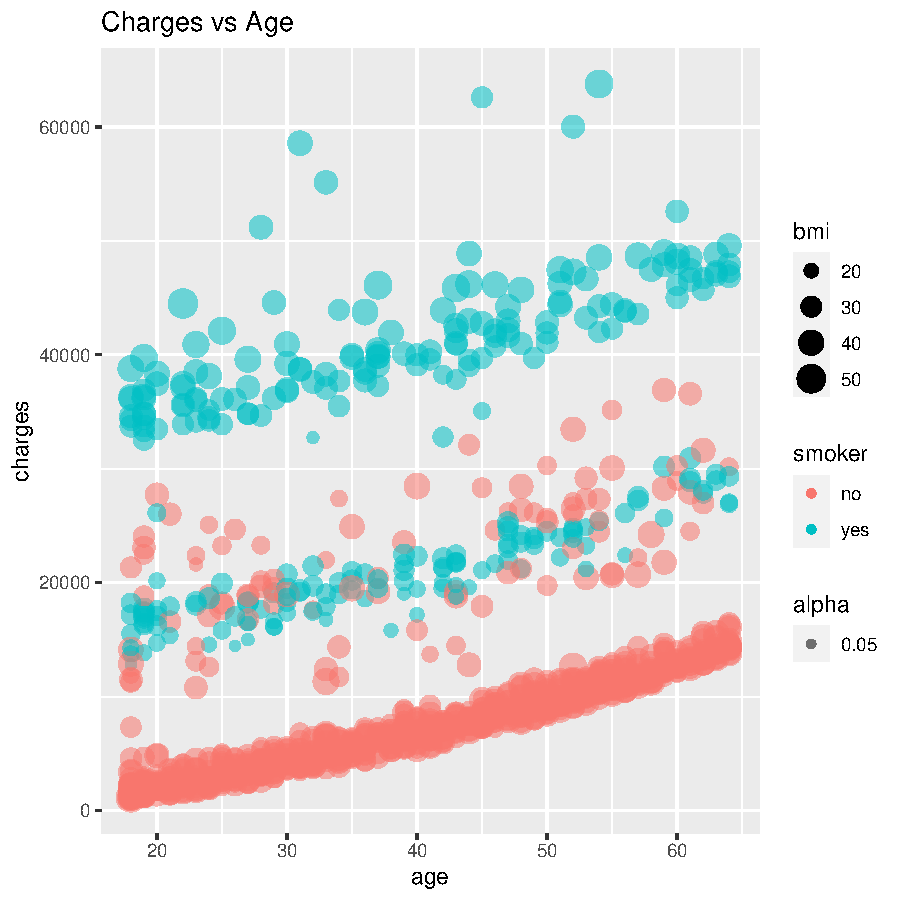
\includegraphics{Untitled-050}
\caption{Age and Charges}
\label{fig:BestPlot}
\end{centerfig}

\begin{Schunk}
\begin{Sinput}
> cor(data$bmi,data$charges)
\end{Sinput}
\begin{Soutput}
[1] 0.198341
\end{Soutput}
\end{Schunk}

Correlation is 0.198 which means that there is a positive correlation between two variables, 
but it is weak and likely unimportant.

Let's divide bmi data into obese and not (More than 30 bmi is obese)

\begin{Schunk}
\begin{Sinput}
> bmiMoreOrLessThan30 <- ifelse(data$bmi>=30,"yes","no")
> ggplot(data = data,aes(bmiMoreOrLessThan30,charges)) + geom_boxplot(fill = c(2:3)) + ggtitle("Obesity")
\end{Sinput}
\end{Schunk}

As we can see there is no big difference in insurance costs, but 
those with high BMI has more outliers, which means hard deseases etc.


\section{Building Regression a model}

Let's build linear model using all possible variables and analyse the result

\subsection{First model}
\begin{Schunk}
\begin{Sinput}
> model_all <- lm(charges ~ age + sex + bmi + children + smoker,data)
> summary(model_all)
\end{Sinput}
\begin{Soutput}
Call:
lm(formula = charges ~ age + sex + bmi + children + smoker, data = data)

Residuals:
     Min       1Q   Median       3Q      Max 
-11837.2  -2916.7   -994.2   1375.3  29565.5 

Coefficients:
             Estimate Std. Error t value Pr(>|t|)    
(Intercept) -12052.46     951.26 -12.670  < 2e-16 ***
age            257.73      11.90  21.651  < 2e-16 ***
sexmale       -128.64     333.36  -0.386 0.699641    
bmi            322.36      27.42  11.757  < 2e-16 ***
children       474.41     137.86   3.441 0.000597 ***
smokeryes    23823.39     412.52  57.750  < 2e-16 ***
---
Signif. codes:  0 '***' 0.001 '**' 0.01 '*' 0.05 '.' 0.1 ' ' 1

Residual standard error: 6070 on 1332 degrees of freedom
Multiple R-squared:  0.7497,	Adjusted R-squared:  0.7488 
F-statistic:   798 on 5 and 1332 DF,  p-value: < 2.2e-16
\end{Soutput}
\end{Schunk}

Analyse the results for group of data to figure out which needs to be removed
And which relationships are the strongest 

Let's remind what those columns mean, and apply it to our results:

\begin{itemize}
  \item \textbf{Standard Error} - measures the average amount 
  that the coefficient estimates vary from the actual average value of our response variable
  \begin{itemize}
    \item \textbf{Expectations} -> lower number relative to estimation coefficients
    \item \textbf{Reality} -> For age and bmi this values are low enough
  \end{itemize}
  \item \textbf{T Value} -> Is a measure of how many standard deviations our coefficient estimate is far away from 0.
  \begin{itemize}
    \item \textbf{Expectations} -> If it is far away from 0, we can reject null-hypothesis (declare that relationship)
    exists
    \item \textbf{Reality} -> For age,bmi and smokers it seems that some kind of relationship exists, but
    The strongest one for a first look is with smokers (Need to mention that we are talking about
    Relationship with Charges)
  \end{itemize}
    \item \textbf{Reality}
  \begin{itemize}
    \item \textbf{Expectations} -> lower number relative to estimation coefficients
    \item \textbf{Reality} -> For age and bmi this values are low enough
  \end{itemize}
  \item \textbf{Pr(> |t|) } -> Relates to the probability of observing any value equal or larger than t.
  In other words, indicates, the possibility of value/relation been observed by chance
  \begin{itemize}
    \item \textbf{Expectations} -> less than 0.05
    \item \textbf{Reality} -> For all except gender is less than 0.05, which satisfies us
  \end{itemize}
    \item \textbf{Residual standard error} -> measure of quality of linear regression fit the data (In other words it is the average amount that the response (age/bmi etc.) will deviate from the true regression line.)
  \begin{itemize}
    \item \textbf{Expectations} -> Lower, comparing with estimate, better.
    Also expecting it to be normal
    \item \textbf{Reality} -> Only for smokers we can see low difference, or about 25\% error on guessing
  \end{itemize}
    \item \textbf{Multiple R-squared} - > Measure of how well the model is fitting the actual data.
  \begin{itemize}
    \item \textbf{Expectations} -> Close to 1
    \item \textbf{Reality} -> 74\% , not bad, but can be better
  \end{itemize}
    \item \textbf{Adjusted R-squared} ->Adjusts Multiple R-squared for the number of variables considered
  \begin{itemize}
    \item \textbf{Expectations} -> Close to 1
    \item \textbf{Reality} -> 0.7488 = 74\%
  \end{itemize}
  \item \textbf{F-statistics} -> indicator of whether there is a relationship between our predictor and the response variables. 
  \begin{itemize}
    \item \textbf{Expectations} -> Further from 1 the better (comparing with data size and predictors)
    \item \textbf{Reality} -> 798
  \end{itemize}
\end{itemize}

\subsection{Second model}
So to start with, I'd remove not really suitable sex and children

\begin{Schunk}
\begin{Sinput}
> model<- lm(charges ~ age + bmi + smoker, data)
> summary(model)
\end{Sinput}
\begin{Soutput}
Call:
lm(formula = charges ~ age + bmi + smoker, data = data)

Residuals:
     Min       1Q   Median       3Q      Max 
-12415.4  -2970.9   -980.5   1480.0  28971.8 

Coefficients:
             Estimate Std. Error t value Pr(>|t|)    
(Intercept) -11676.83     937.57  -12.45   <2e-16 ***
age            259.55      11.93   21.75   <2e-16 ***
bmi            322.62      27.49   11.74   <2e-16 ***
smokeryes    23823.68     412.87   57.70   <2e-16 ***
---
Signif. codes:  0 '***' 0.001 '**' 0.01 '*' 0.05 '.' 0.1 ' ' 1

Residual standard error: 6092 on 1334 degrees of freedom
Multiple R-squared:  0.7475,	Adjusted R-squared:  0.7469 
F-statistic:  1316 on 3 and 1334 DF,  p-value: < 2.2e-16
\end{Soutput}
\end{Schunk}


And now check weather Residual standard error is following normal distribution

\begin{centerfig}
\begin{Schunk}
\begin{Sinput}
> res <- resid(model)
> qqnorm(res)
> qqline(res)
\end{Sinput}
\end{Schunk}
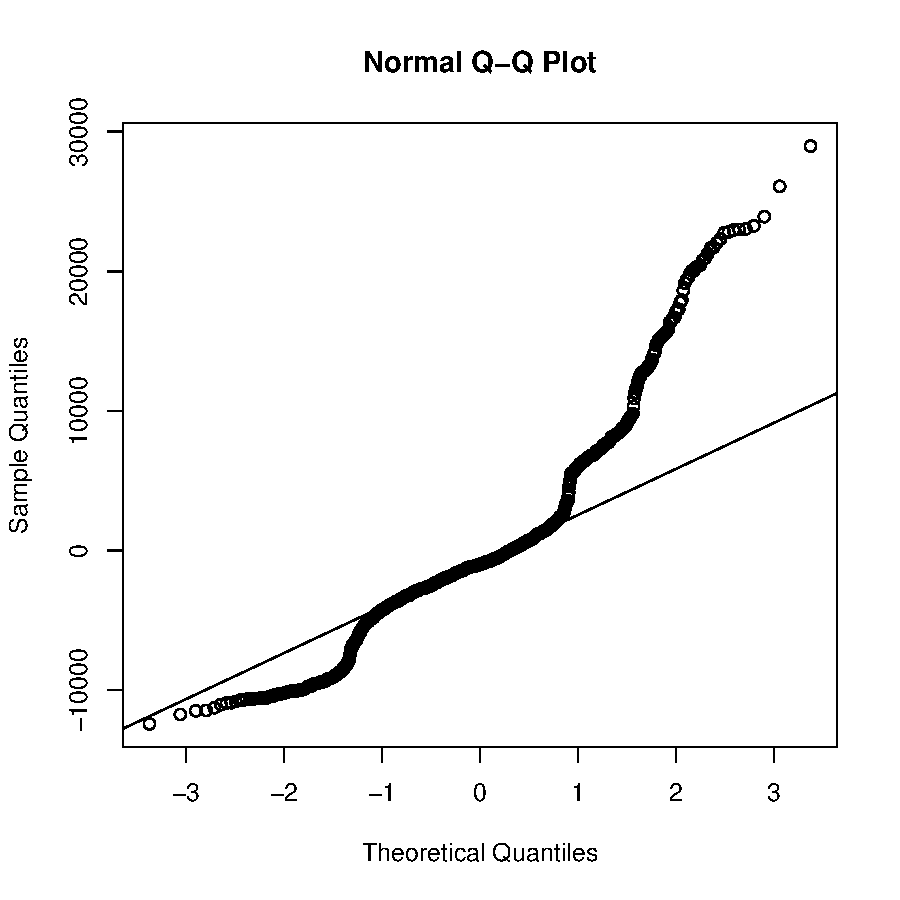
\includegraphics{Untitled-055}
\caption{Residual Standard Error}
\end{centerfig}

As we can see, Residual standard error is not following normal distribution, 
and R-squared can still be better.

\subsection{Third model}
\label{sec:Third}
Now I suggest looking at Smoking closely, because it affects charges the most,
But as we saw in previous analysis, smokers can be devided into two categories
Those with low and high BMI. I suggest us doing that, by adding new variable -> SmokerWithHighBMI

\begin{Schunk}
\begin{Sinput}
> data$SmokerWithHighBMI <- ifelse(data$bmi>30 
+   & data$smoker=="yes","yes","no")
> describeBy(data$charges,data$SmokerWithHighBMI)
\end{Sinput}
\begin{Soutput}
 Descriptive statistics by group 
group: no
   vars    n   mean     sd  median trimmed     mad     min      max    range
X1    1 1194 9842.6 7142.3 8338.75 8863.75 6219.68 1121.87 38245.59 37123.72
   skew kurtosis    se
X1 1.19     1.16 206.7
------------------------------------------------------------ 
group: yes
   vars   n     mean      sd   median  trimmed    mad      min      max
X1    1 144 41692.81 5829.16 40918.31 41225.72 5651.2 32548.34 63770.43
      range skew kurtosis     se
X1 31222.09 1.06     1.78 485.76
\end{Soutput}
\end{Schunk}

Now build the model

\begin{Schunk}
\begin{Sinput}
> model<- lm (charges ~ age  + smoker+ bmi + SmokerWithHighBMI,data)
> summary(model)
\end{Sinput}
\begin{Soutput}
Call:
lm(formula = charges ~ age + smoker + bmi + SmokerWithHighBMI, 
    data = data)

Residuals:
    Min      1Q  Median      3Q     Max 
-5296.9 -1973.2 -1257.8  -398.7 24230.8 

Coefficients:
                      Estimate Std. Error t value Pr(>|t|)    
(Intercept)          -3516.435    738.288  -4.763 2.12e-06 ***
age                    266.328      8.858  30.068  < 2e-16 ***
smokeryes            13593.479    435.742  31.196  < 2e-16 ***
bmi                     47.674     22.031   2.164   0.0306 *  
SmokerWithHighBMIyes 19506.680    590.858  33.014  < 2e-16 ***
---
Signif. codes:  0 '***' 0.001 '**' 0.01 '*' 0.05 '.' 0.1 ' ' 1

Residual standard error: 4521 on 1333 degrees of freedom
Multiple R-squared:  0.8611,	Adjusted R-squared:  0.8607 
F-statistic:  2065 on 4 and 1333 DF,  p-value: < 2.2e-16
\end{Soutput}
\end{Schunk}

Analysing as in previous model, we can come to 
Adjusted R-squared is 85,8\%, which is higher than in previous model
which gives us the possibility to say that data is fitting the model
Errors are lower, t-values are greater, Pr( >|t|) is slightly bigger 
on average, which, makes our results more random, but for all
except BMI it's still less than 0.05, which is normal


Now lets build Residual standard error and check if is 
Following normal distribution

\begin{centerfig}
\begin{Schunk}
\begin{Soutput}
[1] 26326.32
\end{Soutput}
\begin{Soutput}
[1] 26357.51
\end{Soutput}
\end{Schunk}
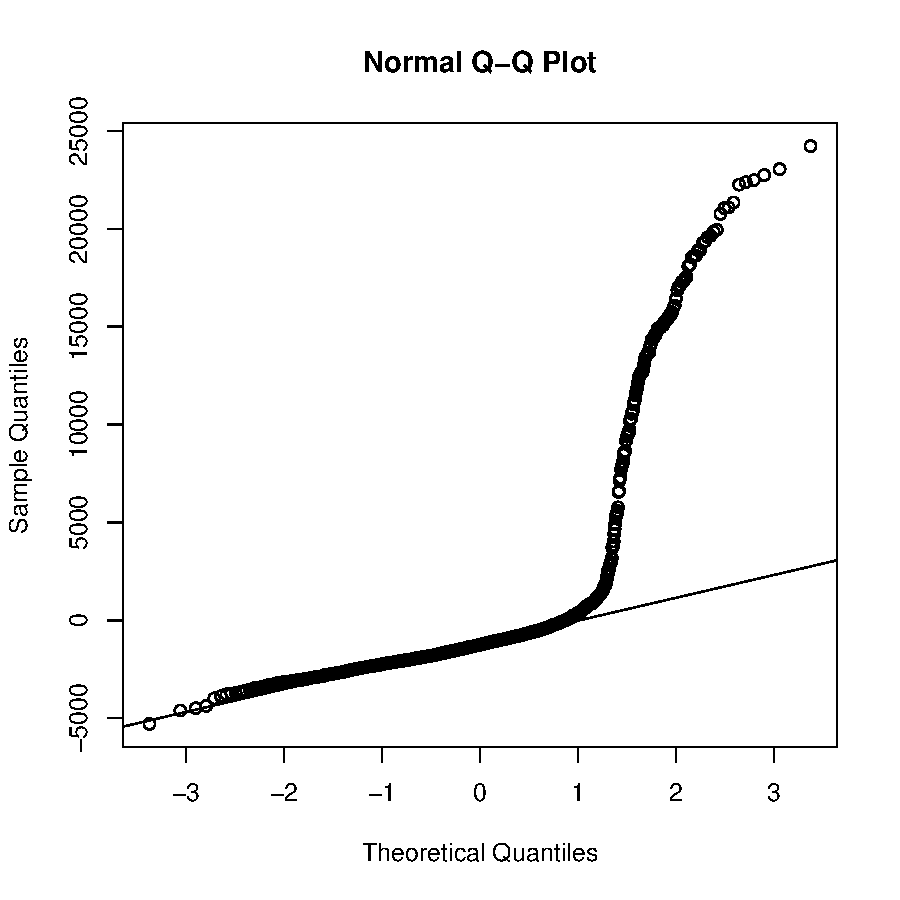
\includegraphics{Untitled-058}
\caption{Residual standard error}
\end{centerfig}

Let's also check for plots of our model parameters

Interpreting of results:
\begin{itemize}
  \item Residuals vs Fitted -> Shows if residuals have non-linear patterns. 
  In our case we have a bit clustered left side which means that there are 
  Some outliers not covered by model 
  \item Normal Q-Q -> Shows if residuals are normally distributed
  As we can see there is a part when data stops following the normal distribution
  Which means that our model doesn't cover all the outliers, and 
  Error while defining them can be significant !!! Which means that we need to work
  More on model
  \item Scale-Location -> The assumption of equal variance
  Data is not spread randomly on the line, which is not quite good
  \item Residuals vs Leverage -> This plot helps us to find influential cases (i.e., subjects) if any. 
  Watch if Cook's distance is high

\end{itemize}


\begin{centerfig}
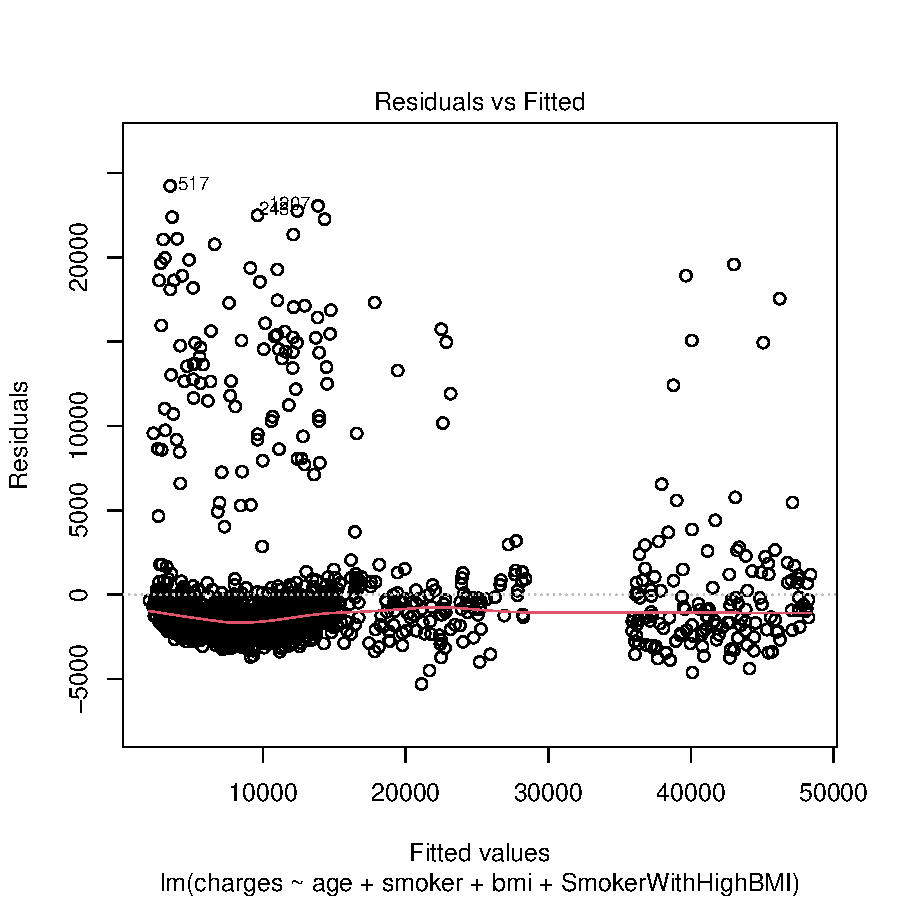
\includegraphics{Untitled-059}
\caption{Residuals vs Fitted}
\end{centerfig}

\begin{centerfig}
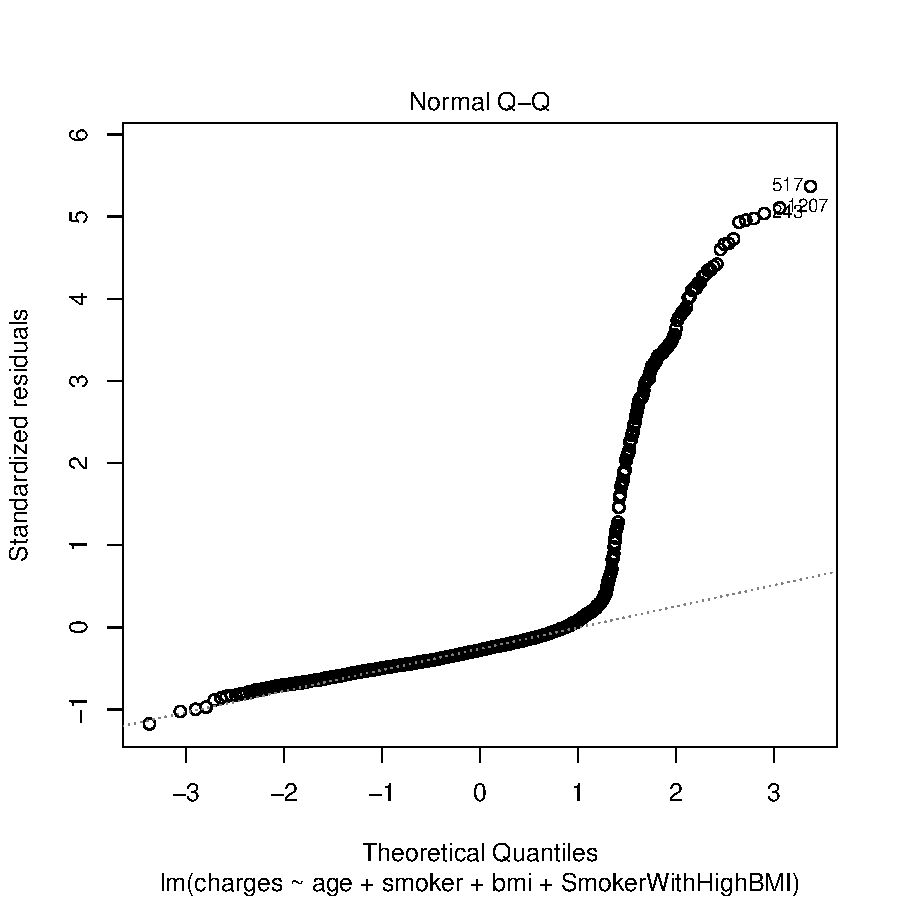
\includegraphics{Untitled-060}
\caption{Normal Q-Q}
\end{centerfig}

\begin{centerfig}
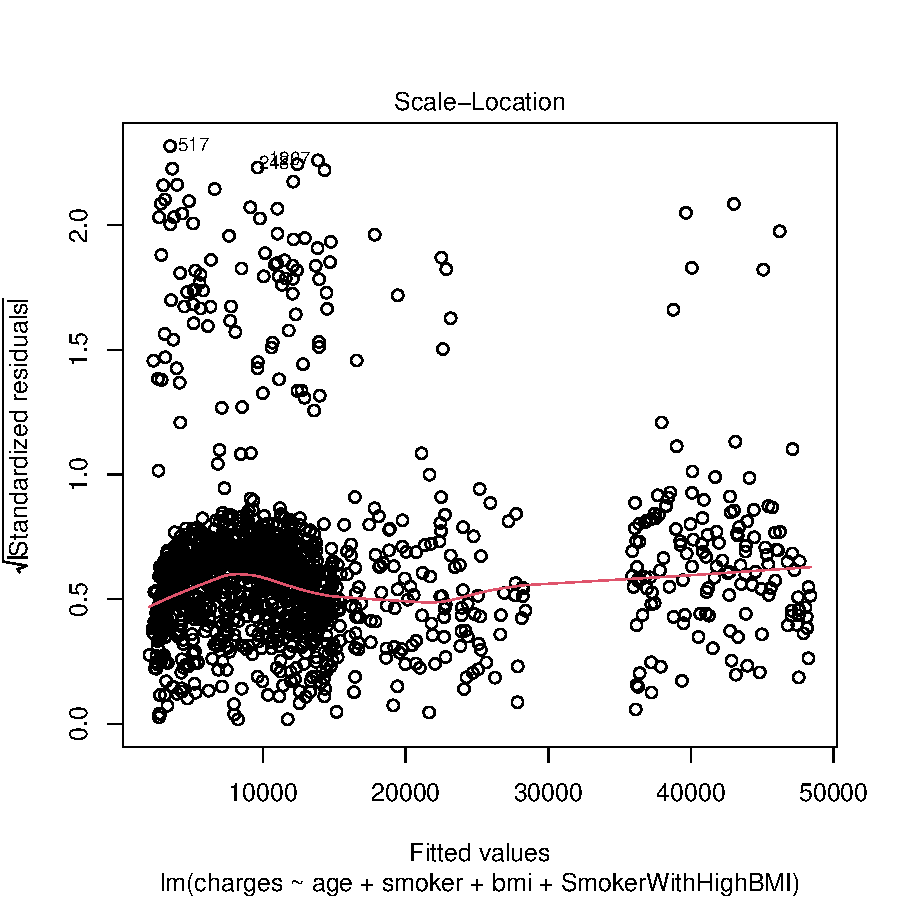
\includegraphics{Untitled-061}
\caption{Scale-Location}
\end{centerfig}


\begin{centerfig}
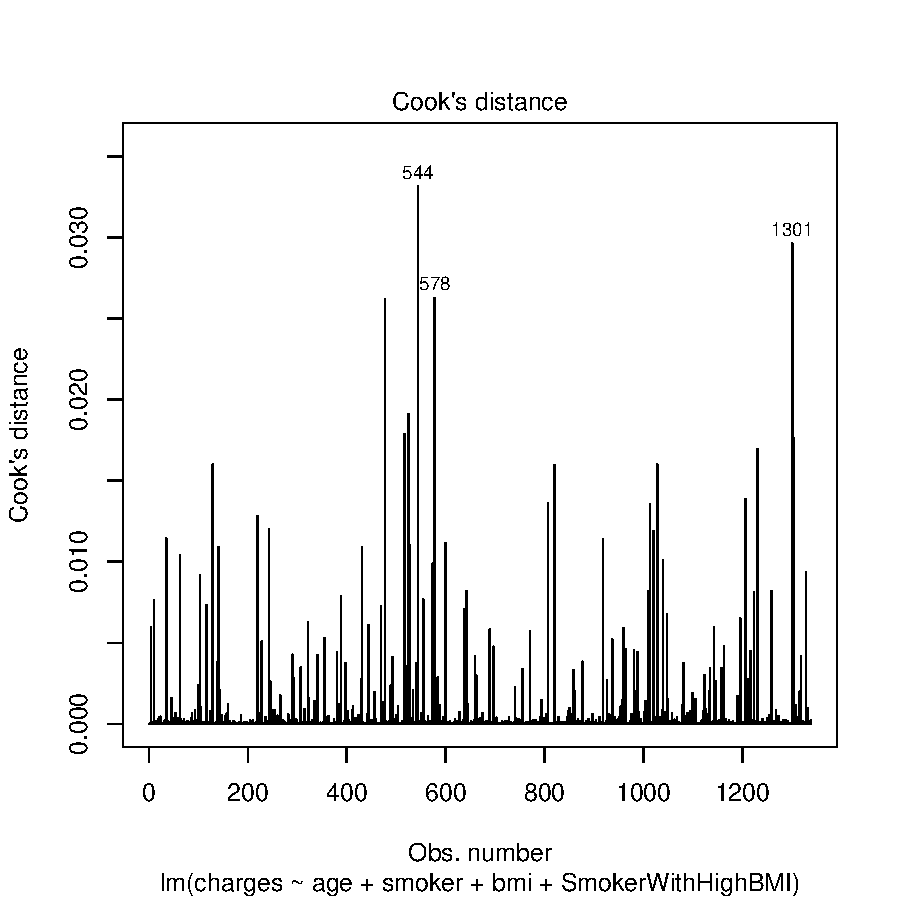
\includegraphics{Untitled-062}
\caption{Residuals vs Leverage}
\end{centerfig}


Because we are not realy satisfied with result, let's search more:

\subsection{Fourth model}
\label{sec:Fourth}
\begin{Schunk}
\begin{Sinput}
> model<- lm (log(charges) ~ age  + age^2 + 
+               smoker+ bmi + SmokerWithHighBMI + children,data)
> summary(model)
\end{Sinput}
\begin{Soutput}
Call:
lm(formula = log(charges) ~ age + age^2 + smoker + bmi + SmokerWithHighBMI + 
    children, data = data)

Residuals:
     Min       1Q   Median       3Q      Max 
-0.90987 -0.17960 -0.04327  0.04700  2.12107 

Coefficients:
                      Estimate Std. Error t value Pr(>|t|)    
(Intercept)          7.2433744  0.0707134  102.43   <2e-16 ***
age                  0.0349966  0.0008428   41.52   <2e-16 ***
smokeryes            1.2155367  0.0414294   29.34   <2e-16 ***
bmi                  0.0018016  0.0020946    0.86     0.39    
SmokerWithHighBMIyes 0.6248198  0.0561753   11.12   <2e-16 ***
children             0.1020739  0.0097599   10.46   <2e-16 ***
---
Signif. codes:  0 '***' 0.001 '**' 0.01 '*' 0.05 '.' 0.1 ' ' 1

Residual standard error: 0.4298 on 1332 degrees of freedom
Multiple R-squared:  0.7824,	Adjusted R-squared:  0.7816 
F-statistic: 957.7 on 5 and 1332 DF,  p-value: < 2.2e-16
\end{Soutput}
\end{Schunk}

\begin{centerfig}
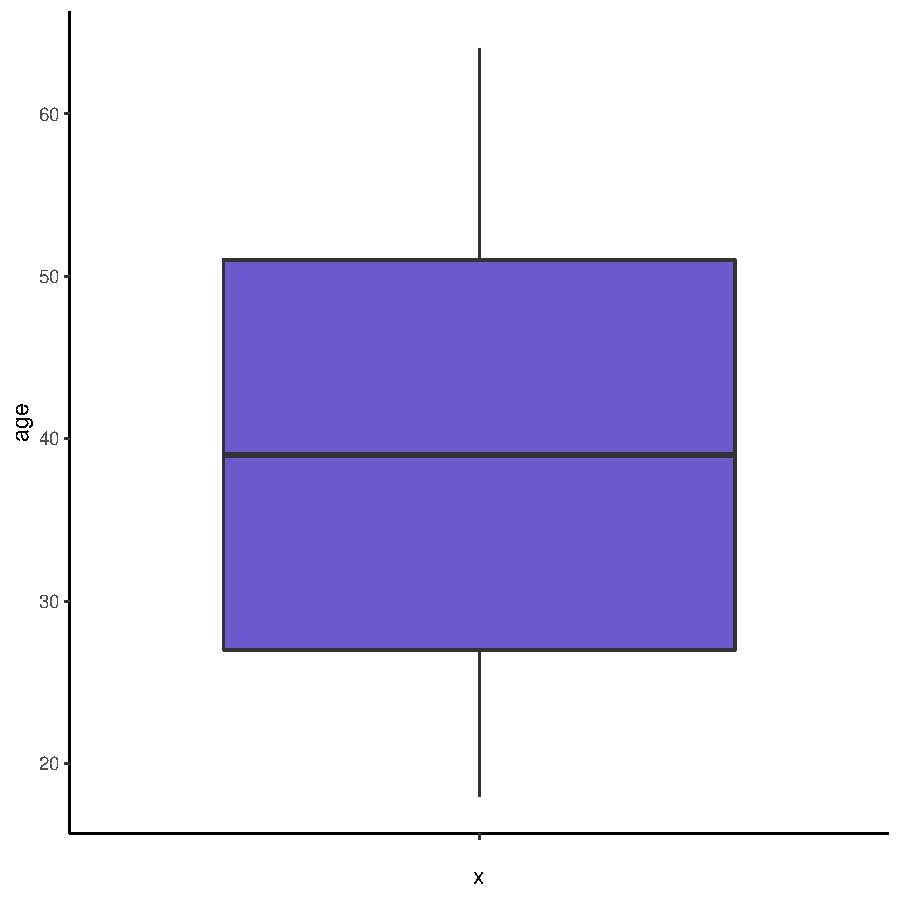
\includegraphics{Untitled-064}
\caption{Residuals vs Fitted}
\end{centerfig}


\begin{centerfig}
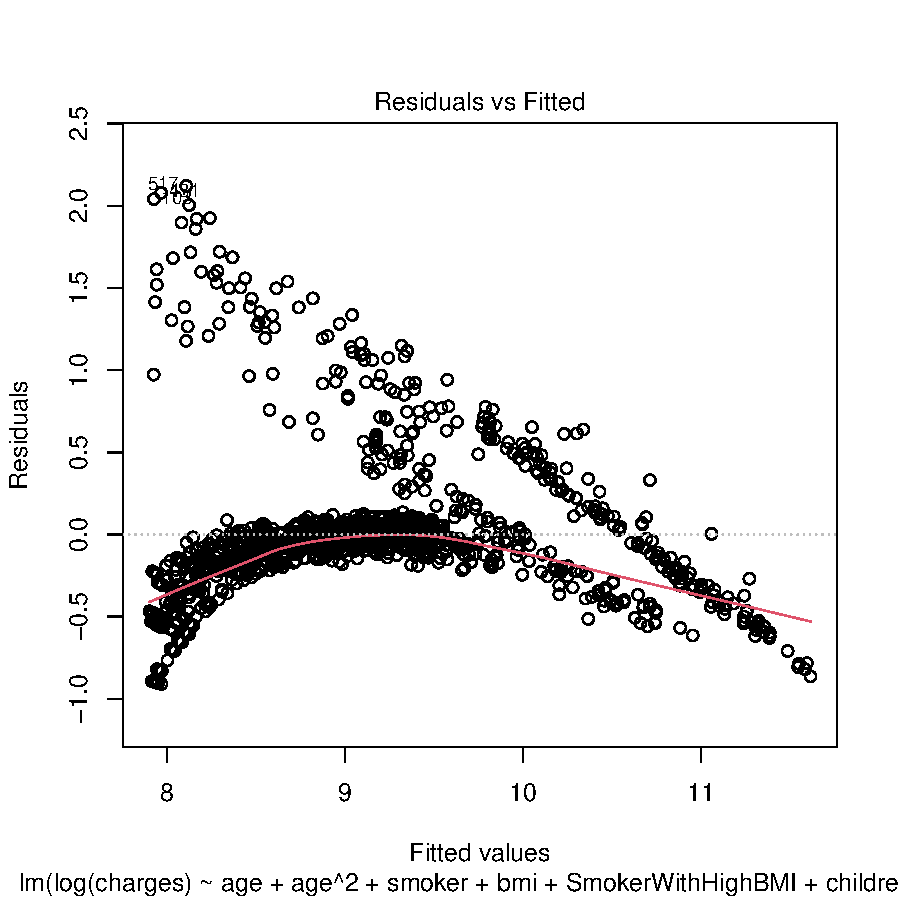
\includegraphics{Untitled-065}
\caption{Residuals vs Fitted}
\end{centerfig}

\begin{centerfig}
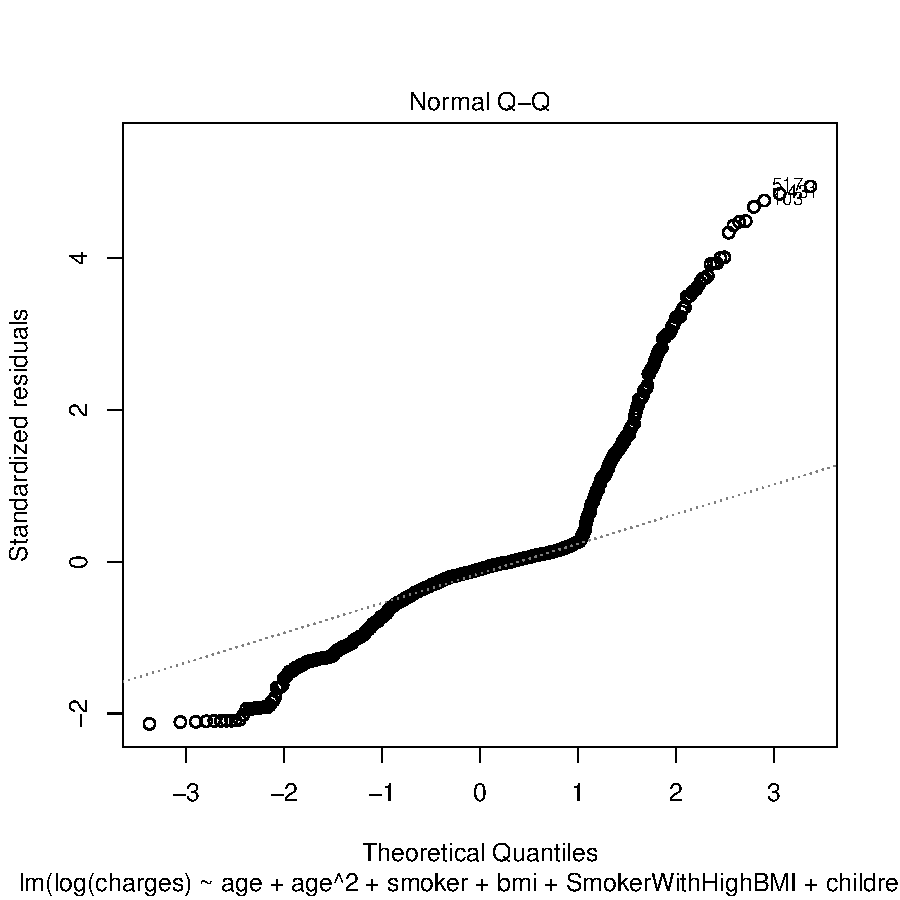
\includegraphics{Untitled-066}
\caption{Normal Q-Q}
\end{centerfig}

\begin{centerfig}
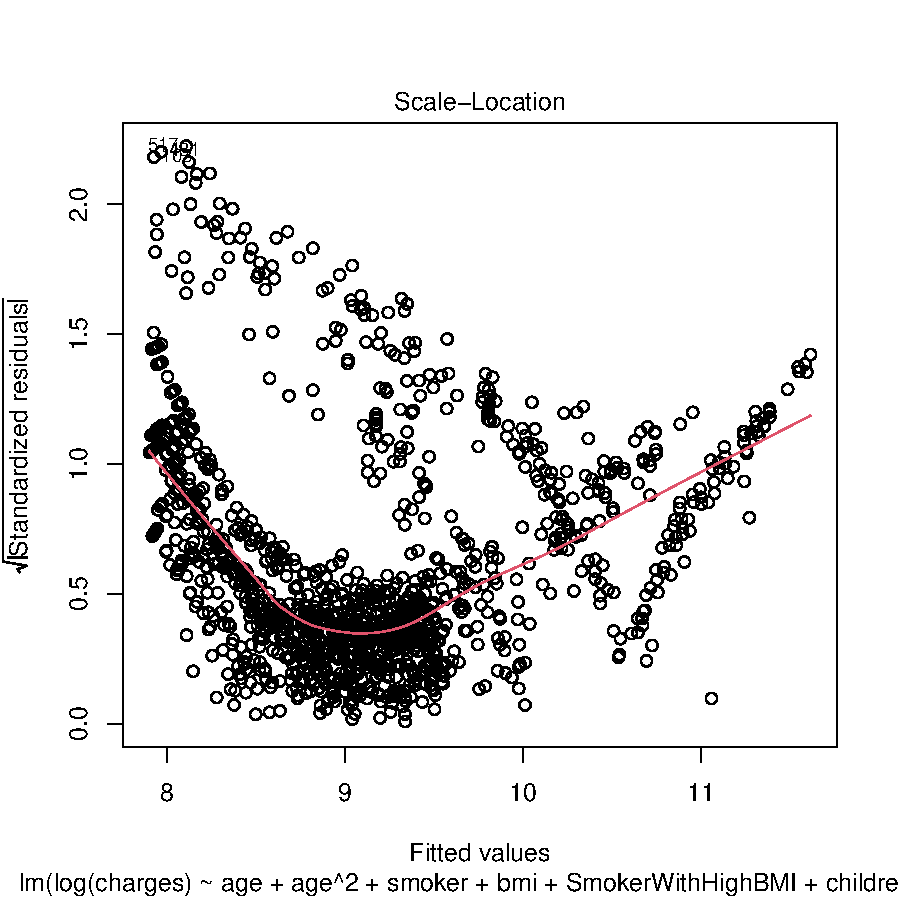
\includegraphics{Untitled-067}
\caption{Scale-Location}
\end{centerfig}


\begin{centerfig}
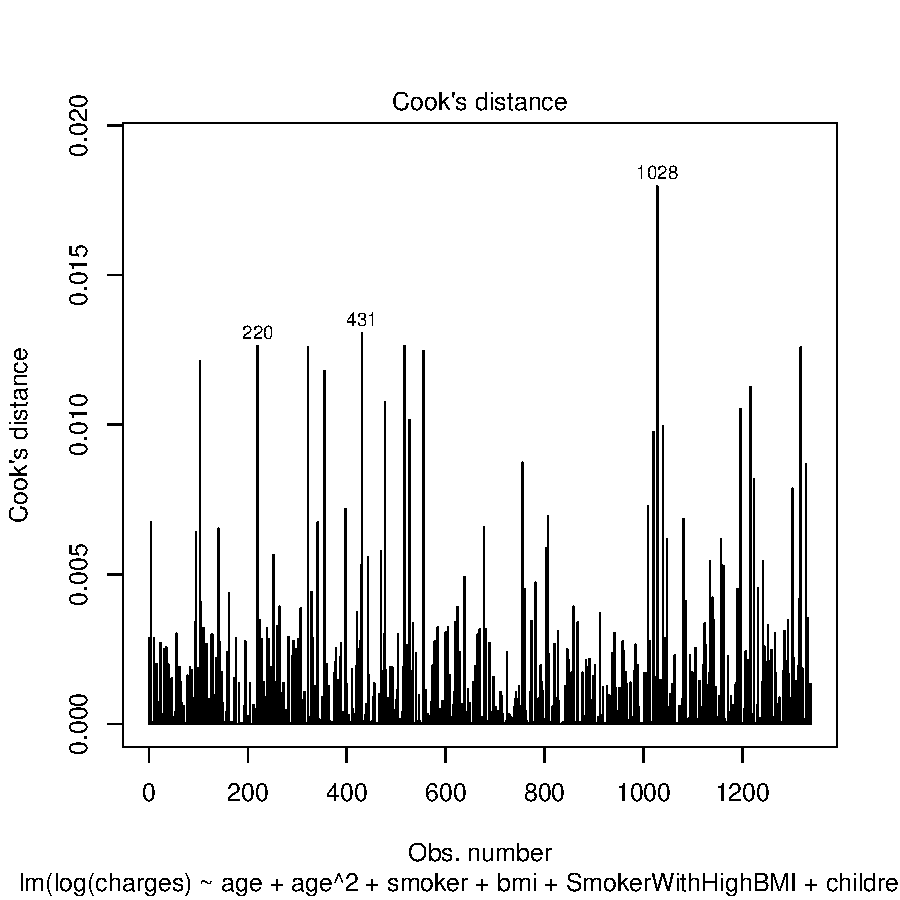
\includegraphics{Untitled-068}
\caption{Residuals vs Leverage}
\end{centerfig}

As we can see, data on graphics is better distributed, but we still have problems with Normal Q-Q, which is not normal  
Residuals are essentially the difference between the actual observed response values. So we need them to be normally distributed across 0




\subsection{Summing up on models}

Choosing the best model from those, that we have built, I would choose the Third One \ref{sec:Third}. Because it has averagely better results comparuing to others, but 
still it doesn't fit all the data, espessially those with high BMI. 



\section{Conclusion}
As we can see on the Figure \ref{fig:BestPlot} there are next dependencies
\begin{itemize}
  \item Charges depend lineary on Age
  \item Charges depend on smoking status, you pay, 2 or 4 (if you also have high BMI) times more than those with middle BMI (around 30) and non-smoking
  \item Charges depend on BMI, but BMI affects less
  \item Charges doesn't depend on gender
\end{itemize}

\end{document}
